
\chapter{Capteurs CMOS pour le d\'etecteur de vertex de l'ILD et pour le projet AIDA}

%Transition chapitre 1.
%On a decrit la physique et les detecteurs ... decrivons les capteurs pour cette physique. 
%Intro : description capteurs, echelles, super-plans pour AIDA. les comprendre pour les simul\'er.
%Comparaison des technos ?? a voir ... description rapide ?

\section{Capteurs CMOS pour le d\'etecteur de vertex de l'ILD}

   Les $APS$ ou Active-Pixel Sensors sont des capteurs imageurs compos\'es d'une matrice de pixels actifs. Les pixels qu'ils contiennent sont d\'enomm\'es actifs car ils contiennent une diode de d\'etection et un amplificateur du signal. Depuis les ann\'ees 1990 les APS se sont d\'evelopp\'es et sont devenus une alternative aux CCD (Charge-Coupled Device). Les APS sont produits gr\^ace au proc\'ed\'e industriel CMOS (Complementary Metal Oxide Semiconductor) et on les retrouve aujourd'hui dans la plupart des appareils photographiques. Les capteurs d\'evelopp\'es dans le groupe PICSEL de l'IPHC sont des MAPS ou \textit{Monolithic Active Pixel Sensor}. Ces capteurs sont dit monolithiques puisque le volume sensible et les circuits micro-\'electroniques qui les composent ne forment qu'un seul objet physique. C'est ainsi que les capteurs developp\'es \`a l'IPHC sont appelés MIMOSA ou \textit{Minimum Ionizing MOS Active pixel sensor}. Le premier des capteurs MIMOSA, nomm\'e MIMOSA-1 a vu le jour en 1999 et les capteurs MIMOSA sont en d\'eveloppement actif depuis cette date. 2013 a vu na\^itre le capteur MIMOSA-34. L'objet de ce chapitre est l'\'etude du fonctionnement et de l'ad\'equation avec les objectifs scientifiques de ces capteurs CMOS.
  
  %description g\'en\'erale \\
  %Capteur pour AIDA \\
  
  \subsection{Contraintes sur les capteurs CMOS}
  \label{sect:contrainte_physiques}
  
   La figure de m\'erite d'un d\'etecteur de vertex est sa r\'esolution sur le param\`etre d'impact $\sigma_{IP}$ c'est-\`a-dire sa résolution sur la distance de plus courte approche de l'h\'elice (la trace) au point d'interaction. La r\'esolution sur le param\`etre d'impact s'exprime de la mani\`ere suivante : 
   
   \begin{equation}
    \sigma_{IP}(p) = a \, \oplus \dfrac{b}{p \, \sin^{\frac{3}{2}}(\theta) }
   \end{equation}

   Le terme $a$ est reli\'e \`a la résolution des capteurs composants le d\'etecteur de vertex. La diffusion multiple est aussi responsable d'une incertitude sur le param\`etre d'impact. Elle est caract\'eris\'ee par le terme $b$. Une expression analytique des param\`etres $a$ et $b$ pour un d\'etecteur de vertex \'equip\'e de deux couches, une interne et une externe, le tout avec des traces droites (d'impulsion infinie) est la suivante :
   
   \begin{equation}
    a = \sqrt{ \left( \dfrac{R_{ext}}{R_{ext}-R_{int}} \right)^2 \sigma_{int}^2 + \left( \dfrac{R_{int}}{R_{ext}-R_{int}} \right)^2 \sigma_{ext}^2 }
   \end{equation}
   
   \begin{equation}
    b = R_{int} 13.6 \, \, MeV/c \, Z \, \sqrt{\dfrac{x}{X_0}} \left(1 + 0.038  \, ln \left(\dfrac{x}{X_0 \sin(\theta)}\right) \right)
   \end{equation}

   Avec $R_{int}$ le rayon de la couche interne, $R_{ext}$ le rayon de la couche externe, $\sigma_{int}$ et $\sigma_{ext}$ respectivement les r\'esolutions des capteurs \'equipant les couches internes et externes, $Z$ la charge de la particule traversant le d\'etecteur de vertex, et $x$ et $X_0$ respectivement l'\'epaisseur et la longueur de radiation du mat\'eriau travers\'e.
   
   \medskip
   
   Dans cette configuration, le param\`etre $a$ est donc principalement fix\'e par la r\'esolution des capteurs du d\'etecteur de vertex et par les rayons des couches qui le composent. Le param\`etre $b$ est quant \`a lui reli\'e au budget de mati\`ere (terme $x/X_0$) mais aussi au rayon de la premi\`ere couche de d\'etection du d\'etecteur de vertex.
   
   \medskip
   
   L'ILD devra \^etre \'equip\'e d'un d\'etecteur de vertex ayant comme param\`etres : $a \leq 5 \, \mu m$ et $b \leq 10 \, \mu m \, GeV/c$. Des valeurs aussi basses n'ont jamais \'et\'e atteintes par le pass\'e comme l'atteste le tableau \ref{tab:AB} repr\'esentant les param\`etres $a$ et $b$ pour les quelques détecteurs de vertex représentatifs en physique des particules et pour celui de l'ILC.
   
  \begin{table}[h]
   \begin{center}
    \begin{tabular}{|l|l|l|} \hline
     Collisionneur & $a$ ($\mu m$) & $b$ ($\mu m \, GeV/c$) \\ \hline
     LEP           & 25          & 70                   \\ \hline
     SLC           & 8           & 33                   \\ \hline
     LHC           & 12          & 70                   \\ \hline
     RHIC          & 13          & 19                   \\ \hline
     ILC           & $\leq 5$    & $\leq 10$            \\ \hline
    \end{tabular}
    \caption{Param\`etres $a$ et $b$ de la r\'esolution sur le param\`etre d'impact de quelques détecteurs représentatifs des collisionneurs de particules.}
    \label{tab:AB}
   \end{center}
  \end{table}

  \medskip
  
  Comme nous l'avons déjà vu \hyperref[list:caracteristiques]{pr\'ec\'edemment} (Chapitre \ref{sect:paramVTX}) les caract\'eristiques requises pour les capteurs composant le d\'etecteur de vertex de l'ILD devront répondre au cahier des charges suivant : 
  
  \medskip
  
   \renewcommand{\labelitemi}{$\bullet$}
  \begin{itemize}
   \item Une r\'esolution spatiale proche du point d'interaction $\leq$ 3 $\mu m$
   \item Un budget de mati\`ere inf\'erieur \`a $0.15 \%$ $X_0$ par couche
   \item Une premi\`ere couche \`a environ 16 $mm$ du point d'impact.
   \end{itemize}
  
  \medskip
  
  Le rayon de la premi\`ere couche de d\'etection est limit\'e par le rayon du tube du faisceau valant 14 $mm$. Une premi\`ere couche de d\'etection situ\'ee \`a une distance d'environ 16 $mm$ du point d'interaction coupl\'ee à une r\'esolution spatiale des capteurs la composant permettra d'atteindre les pr\'e-requis sur le param\`etre $a$. Quant au param\`etre $b\leq10$, celui-ci devrait être atteint gr\^ace \`a un budget de mati\`ere pour les échelles composant les couches du d\'etecteur de vertex inf\'erieur ou \'egale \`a $0.15 \%$ $X_0$, c'est \`a dire inf\'erieur ou \'egale \`a $0.30 \%$ $X_0$ pour une couche \'equipée de capteurs sur ses deux faces. Un tel budget de mati\`ere n'a pour l'instant pas \'et\'e atteint. Les prototypes d'échelles actuels proposent un budget de mati\`ere 2 fois sup\'erieur \`a ces pr\'e-requis.
  
%   \subsubsection{Efficacit\'e de d\'etection}
% 
%    \subsubsection{Vitesse de lecture}
%    \subsubsection{Puissance consomm\'ee}
%    \subsubsection{Tol\'erance aux radiations}
% 
%   \subsubsection{Taux d'occupation}
%   \subsubsection{Distinction des co\^uts}
  
%  La physique et les implications sur les capteurs CMOS \\
%  -temps de lecture -> suppression de zero -> rolling shuter \\
%  -resolution/pitchs des pixels \\
%  -Puissance dissip\'ee (rolling shuter) (voir hdr jerome )
%  Schema qui va bien ("quadrature des Pixels CMOS")
 
%  vertexing \\ 
%  parametre a et b -> budget de matiere, resolution ... \\
  
  \subsection{Fonctionnement des capteurs CMOS}
  
  Nous allons \`a pr\'esent d\'ecrire le fonctionnement des capteurs CMOS pour la physique des particules.
  
  \subsubsection{D\'epôt d'\'energie dans le capteur}
  \label{sect:bethe_bloch}
    % Mimosa 22 ?
    % particule minimum d'ionisation ? parce que plat apres 750 MeV/c ?
    % Bethe Block OK
    % Pourquoi une Landau ? OK
    % Comment a-t-on mesur\'e 80 e-/µm ?
 
    Lors de son parcours dans la mati\`ere, une particule charg\'ee interagit avec les électrons et les noyaux des atomes du milieu et perd de l'\'energie. La plupart des interactions mises en jeux sont des collisions quasi-élastiques. Ces collisions peuvent provoquer l'ionisation d'un atome ou l'excitation de ce dernier. L'\'energie transf\'er\'ee au noyau restant g\'en\'eralement tr\`es faible.
    
    \medskip
    
    La perte moyenne d'\'energie dans la mati\`ere par unit\'e de longueur est donn\'ee par la relation de Bethe et Bloch :
    
    \[ -\cfrac{dE}{dx} = 4 \pi N_A r_e^2 m_e c^2 z^2 \cfrac{Z}{A} \cfrac{1}{\beta^2} \left[ \cfrac{1}{2} \, ln\left( \cfrac{2 m_e c^2 \beta^2 \gamma^2 T_{max} }{I^2} \right) - \beta^2 -\cfrac{\delta}{2} \right]  \]
 
    o\`u $N_A$ est le nombre d'Avogadro, $r_e$ le rayon classique de l'\'electron, $m_e$ la masse de l'\'electron, $z$ la charge de la particule incidente, $A$ et $Z$ respectivement le num\'ero atomique et le nombre de masse du milieu travers\'e, $\beta$ et $\gamma$ les facteurs de Lorentz de la particule, $T_{max}$ l'\'energie maximale pouvant \^etre transf\'er\'ee \`a un \'electron d'ionisation et I l'\'energie moyenne d'excitation du milieu. $\delta$ symbolise les effets densit\'e.
    
    Pour une particule de masse $M$, $T_{max}$ vaut :
    
    \[ T_{max} = \cfrac{2 m_e c^2 \beta^2 \gamma^2}{1 + 2 \gamma m_e/M + (m_e/M)^2} \]

   Une partie de l'\'energie perdue par la particule incidente provient de l'\'emission de rayons $\delta$ et de photons. Pour une couche finie de mat\'eriau, ces particules peuvent traverser tout le milieu, et en sortir, tout en ne d\'eposant qu'une part de leur \'energie. Pour tenir compte de cet effet dans le processus d'ionisation et d'excitation, on limite $T$, l'\'energie transf\'er\'ee \`a un \'electron d'ionisation, de sorte que $T \leq T_{cut} \leq T_{max}$. On obtient alors la relation de Bethe et Bloch modifi\'ee suivante :
   
   \[ -\cfrac{dE}{dx} = 4 \pi N_A r_e^2 m_e c^2 z^2 \cfrac{Z}{A} \cfrac{1}{\beta^2} \left[ \cfrac{1}{2} \, ln\left( \cfrac{2 m_e c^2 \beta^2 \gamma^2 T_{cut} }{I^2} \right) - \cfrac{ \beta^2 }{2} \left( 1 + \cfrac{T_{cut}}{T_{max}} \right) -\cfrac{\delta}{2} \right]  \]

   La figure ~\ref{fig:restricted_Bethe_Bloch} montre la valeur du pouvoir d'arrêt et le pouvoir d'arrêt restreint pour un Pion dans le silicium en fonction de l'impulsion du Pion.

   \begin{figure}[!htb]
    \begin{center} 
     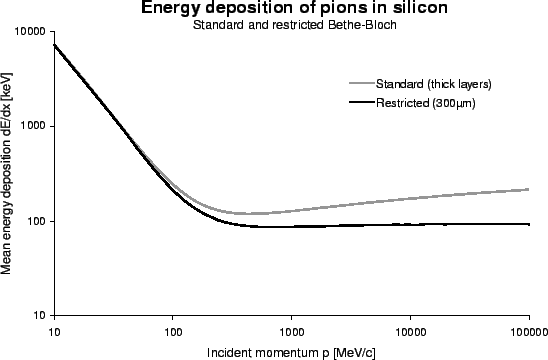
\includegraphics[scale=0.50]{./figures/restricted_Bethe_Bloch.png}
     \caption{Pouvoir d'arrêt et pouvoir d'arrêt restreint pour un Pion dans le silicium.}
     \label{fig:restricted_Bethe_Bloch}
    \end{center}
   \end{figure}   
   
   \medskip
   
   Les relations de Bethe et Bloch ne permettent de calculer que la perte moyenne d'énergie d'une particule traversant un mat\'eriau. Selon le chemin qu'elle parcourt, la particule engendre un nombre de collisions ; et une quantit\'e d'\'energie lib\'er\'ee par collision, variables. La perte d'\'energie suit donc une distribution pour des \'epaisseurs de mat\'eriau finies. Plus l'\'epaisseur du mat\'eriau travers\'ee est importante, plus la distribution de perte d'\'energie tend vers une \textit{gaussiene}. A contrario, plus l'\'epaisseur est fine, plus la distribution tend vers une distribution de \textit{Landau}. Dans notre cas l'\'epaisseur de mat\'eriau sensible travers\'ee, c'est-\`a-dire l'\'epaisseur de la couche épitaxiée est de l'ordre de 15 $\mu m$. La distribution de perte d'\'energie dans le silicium peut alors \^etre approximée par une distribution de \textit{Landau}.
  
  \medskip

   Une estimation r\'ealis\'ee par le groupe \textit{PICSEL}, a montr\'e que la valeur la plus probable (MPV) du d\'epôt de charge le long de la couche épitaxiée pour des pions dot\'es d'une impulsion de 120 $GeV/c$ (SPS) \'etait d'environ $80 \, e^-/\mu m$.
  
  \subsubsection{Principe de fonctionnement}
  
  La structure d'un capteur CMOS et son principe de fonctionnement sont illustr\'es en figure ~\ref{fig:principe}. Un substrat de silicium fortement dop\'e P est tout d'abord cr\'e\'e. Celui-ci est compos\'e de silicium de qualit\'e mod\'er\'ee c'est-\`a-dire qu'il poss\`ede beaucoup de d\'efauts dans sa structure cristalline. Cela engendre un fort taux de recombinaisons des porteurs de charge qui diffusent dans cette couche. Au dessus du substrat, une couche \'epitaxi\'ee d'un faible dopage P est d\'epos\'ee. Cette couche \'epitaxi\'ee est de haute qualit\'e et constitue la couche sensible de notre d\'etecteur. La qualit\'e doit \^etre \'elev\'ee afin de r\'eduire le nombre de recombinaisons des porteurs de charge. La "collection" des charges est effectu\'ee par des caissons N-Well impl\'ement\'es \`a la surface de la couche \'epitaxi\'ee. Ces caissons N forment des jonctions P-N entre la couche \'epitaxi\'ee et les caissons N. Les caissons N repr\'esentent les pixels et on appellera la distance entre deux de ces caissons : \textit{pas inter-pixel}. Autour des caissons N se trouvent des zones P-well fortement dop\'ees. Ce fort dopage cr\'ee une barri\`ere de potentiel entre la couche \'epitaxi\'ee et la zone P-Well. Ainsi les porteurs de charge sont r\'efl\'echis au niveau de cette interface. Il en est de m\^eme pour la zone de transition entre substrat et couche \'epitaxi\'ee. 
  
  \begin{figure}[!htb]
   \begin{center} 
    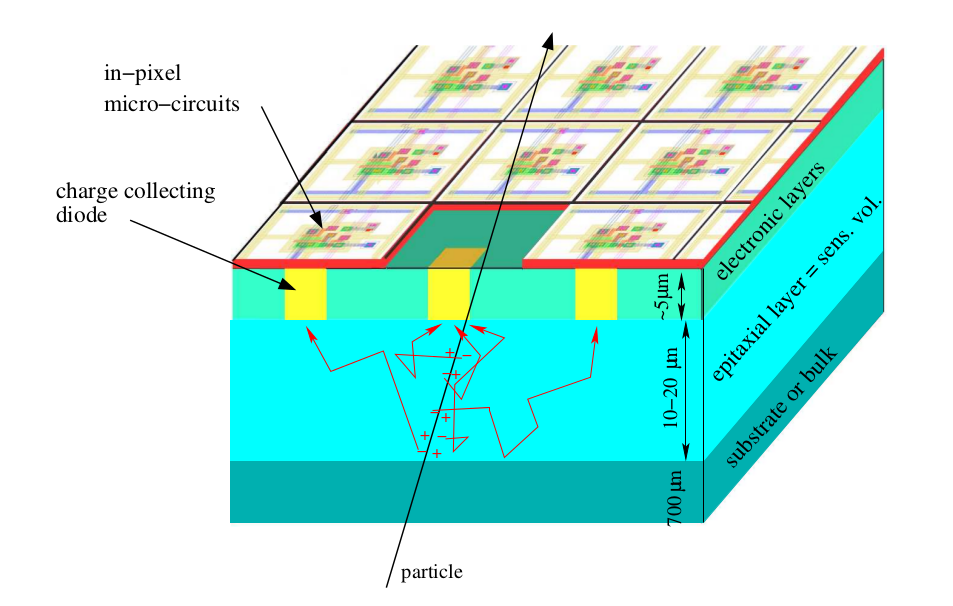
\includegraphics[scale=0.40]{./figures/schema_principe_CMOS.png}
    \caption{Sch\'ema de la structure d'un capteur CMOS et principe de fonctionnement.}
    \label{fig:principe}
   \end{center}
  \end{figure}
  
  \medskip
  
  Les valeurs des dopages pour les diff\'erentes zones sont de l'ordre de $10^{15}$ $at/cm^3$ pour la couche \'epitaxi\'ee, $10^{19}$ $at/cm^3$ pour le substrat et $10^{17}$ $at/cm^3$ pour les zones P-Well. L'interface entre un caisson N et la couche \'epitaxi\'ee cr\'ee une zone d\'epl\'et\'ee qui va attirer les porteurs de charge vers elle. Cette zone est r\'eduite du fait du faible dopage de la couche epitaxi\'ee. Ainsi, la couche \'epitaxi\'ee est majoritairement non d\'epl\'et\'ee. Au passage d'une particule charg\'ee, les diff\'erentes couches sont ionis\'ees, les porteurs de charge diffusent alors thermiquement. Ceux-ci sont fortement recombin\'es dans les zones de structure cristalline m\'ediocres. Dans la couche \'epitaxi\'ee faiblement dop\'ee, les porteurs de charges diffusent et ne sont que très faiblement recombin\'es. Puis, lorsque les porteurs de charge approchent une zone d\'epl\'et\'ee, ils sont attir\'es vers les caissons N, qui collectent les charges.
  
  \medskip
  
  La barri\`ere de potentiel aux interfaces couche \'epitaxi\'ee/substrat et zones P-Well/couche \'epitaxi\'ee est donn\'ee par la relation suivante : 
  
  \begin{equation}
   V = \dfrac{kT}{q} \ln \left( \dfrac{N_{sub}}{N_{epi}} \right)
  \end{equation}
   
   pour l'interface substrat/couche \'epitaxi\'ee et par : 
   
  \begin{equation}
   V = \dfrac{kT}{q} \ln \left( \dfrac{N_{P-Well}}{N_{epi}} \right)
  \end{equation}
   
   pour l'interface zones P-Well/couche \'epitaxi\'ee. O\`u $k$ est la constante de Boltzmann, $q$ la charge de l'\'electron, $T$ la temp\'erature absolue et $N_{sub}$, $N_{epi}$ et $N_{P-Well}$ sont respectivement les dopages du substrat, de la couche \'epitaxi\'ee et des zones P-Well.
   
   \medskip
   
   Comme les porteurs de charges sont diffus\'es thermiquement, leurs parcours moyen \`a travers la couche \'epitaxi\'ee est beaucoup plus long que ceux des porteurs de charge dans un capteur enti\`erement d\'epl\'et\'e. Ainsi la probabilit\'e de recombinaison augmente pour un capteur non d\'epl\'et\'e. L'efficacit\'e de collection de charge pour un capteur non d\'epl\'et\'e est donc inf\'erieure. De plus, les charges sont plus \'etal\'ees ce qui m\`ene \`a un nombre de charges par pixel moins important et plus de pixels touch\'es. Le chemin parcouru par les porteurs de charge \'etant plus long que celui d'un capteur enti\`erement d\'epl\'et\'e, la dur\'ee de collection de charge s'agrandit aussi. Elle est de l'ordre de 100 $ns$.

  \subsubsection{Caract\'eristiques}
  
  Les capteurs CMOS offrent des caract\'eristiques int\'eressantes pour la physique des hautes \'energies et notamment pour la reconstitution des vertex et des traces. Ils permettent un budget de mati\`ere restreint pour une r\'esolution spatiale accrue tout en ayant une bonne tol\'erance aux radiations et un co\^ut de fabrication faible.
  
  \paragraph{R\'esolution spatiale}
  
  Les proc\'ed\'es CMOS poss\`edent une taille de grille de plus en plus fine. Ainsi, une taille de grille inf\'erieure \`a 100 $nm$ est actuellement accessible. La taille minimale d'un pixel est environ un ordre de grandeur au dessus de la taille de grille. Ainsi une taille de diode de l'ordre de quelques $\mu m^2$ est accessible autorisant un pas inter-pixel de l'ordre de la dizaine de microns. En prenant en compte la r\'epartition des porteurs de charge dans les pixels, on peut atteindre une r\'esolution spatiale inf\'erieure au micron. Par exemple on atteint une resolution inf\'erieure ou \'egale au micron pour un pas inter-pixel $\lesssim$ 10 $\mu m$ et sortie analogique. Pour une sortie binaire, par exemple, une r\'esolution de 2.8 \`a 3.0 microns est attendue pour un pas inter-pixel de 17 $\mu m$.
  
  \paragraph{Budget de mati\`ere}
  
  Dans un capteur CMOS seule la couche \'epitaxi\'ee est utilis\'ee pour g\'en\'erer le signal. Les porteurs de charge sont r\'efl\'echis par l'interface entre la couche \'epitaxi\'ee et le substrat. Pour cette r\'eflexion, seule l'interface compte. Ainsi, un amincissement du substrat est permis. Lors de sa conception, ce dernier est g\'en\'eralement dot\'e d'une \'epaisseur de quelques centaines de microm\`etres. Le capteur peut alors \^etre aminci jusqu'à une \'epaisseur de 50 $\mu m$ (voire 30 $\mu m$). Cette taille permet de garder une solidit\'e suffisante pour manipuler le capteur.
  
  \paragraph{Signal}
  
  La taille modeste de la couche \'epitaxi\'ee induit un signal faible au niveau des diodes de collection de charge. Une particule dans son minimum d'ionisation produira environ 80 paires \'electron-trou par $\mu m$ travers\'e ce qui conduit \`a un signal total de l'ordre de 1000 \`a quelques milliers d'\'electrons.

  \paragraph{Coût et fabrication}
  
  Le proc\'ed\'e de fabrication CMOS \'etant un proc\'ed\'e industriel, le co\^ut de revient de cette technologie est moindre. Ce proc\'ed\'e industriel permet un rythme de soumission plus \'elev\'ee que dans le cas d'une technologie non industrielle. Ainsi, plus de prototypes peuvent être con\c{c}us dans le but d'optimiser les capteurs d\'evelopp\'es. Cela permet aussi de pouvoir construire des capteurs de grandes surfaces.
  
  \paragraph{Tol\'erance aux radiations}
  \label{sect:tolrerance_rad}
  Les capteurs CMOS sont sensibles aux rayonnements ionisants et non-ionisants. Les rayonnements ionisants sont responsables de l'accumulation de charges dans les composants des pixels. Ces charges peuvent augmenter le courant de fuite du pixel et de sa diode de collection. Plus la diode sera petite, plus les effets des rayonnements ionisants seront faibles. La solution est donc de réduire la taille des diodes en utilisant une taille de grille la plus faible possible lors de la conception du capteur. Cependant plus la taille de grille est fine plus le co\^ut de revient est \'elev\'e. Les rayonnements non ionisants vont quant \`a eux cr\'eer des dommages au r\'eseau cristallin de la couche \'epitaxi\'ee. Ces dommages vont induire un plus fort taux de recombinaison ce qui implique une baisse du signal. Cette perte de signal est d'autant plus forte que le libre parcours des charges est grand. Une solution pour compenser la perte de signal est de r\'eduire le temps de collection de charge et donc le libre parcours moyen des porteurs de charge. Pour cela 2 solutions peuvent \^etre envisag\'ees : la réduction du pas inter-pixel ou l'augmentation de la r\'esistivité de la couche \'epitaxi\'ee. Cette dernière option permet une augmentation de la zone d\'epl\'et\'ee et donc une diminution du libre parcours moyen des porteurs de charge.
  
  %comparaison avec autre technologies. \\
  %Pourquoi des capteurs CMOS ? Pour quelles applications ?. \\
  
  \subsubsection{Pixels}
  
  \begin{figure}[!htb]
    \begin{center}
      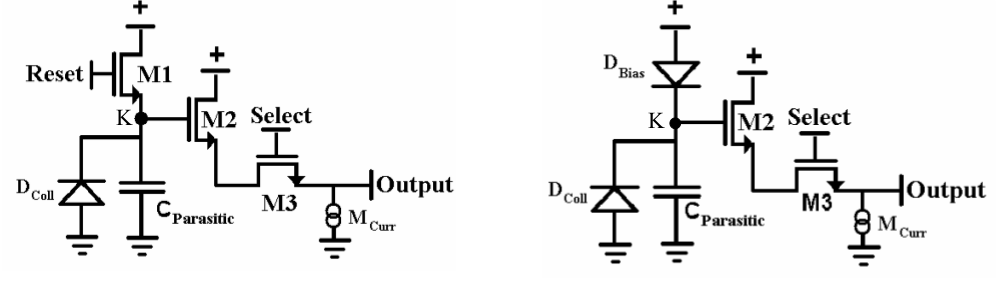
\includegraphics[scale=0.5]{./figures/pixel_transistors.png}
      \caption{\`A gauche, sch\'ema d'un pixel de type \textit{3T}. \`A droite sch\'ema d'un pixel de type Self Biased.}
      \label{fig:pixel_transistor}
    \end{center}
  \end{figure}
  
  Deux types de pixels peuvent \^etre utilis\'es pour les pixels des capteurs CMOS pour la physique des particules. Il s'agit des pixels de type \textit{3T} et des pixels de type \textit{Self-Biased}. La figure \ref{fig:pixel_transistor} illustre les deux types de pixels.
  
  \paragraph{3T} Les pixels de type \textit{3T} fonctionnent en 2 grandes phases. La premi\`ere phase est constitu\'ee par une premi\`ere lecture du pixel puis une seconde lecture espac\'ee du temps d'int\'egration du capteur. Durant cette phase d'int\'egration le pixel est sensible et il accumule les charges pr\'esentes. Le transistor $M1$ (voir figure) est alors ferm\'e. Toujours, durant cette phase, la capacit\'e $C$ du pixel diminue l\'eg\`erement \`a cause du courant de fuite. Il faut alors compenser ce courant de fuite. Pour cela la seconde phase d\'ebute avec un signal de mise \`a zéro (\textit{reset}) qui ouvre le transistor $M1$. Cela a pour effet de recharger la capacit\'e du pixel. Le courant de fuite est ainsi compens\'e jusqu'à la prochaine remise \`a z\'ero. L'\'etape de remise \`a z\'ero coûte parfois jusqu'\`a 50 $\%$ du temps de lecture. Il serait alors judicieux d'\'eviter cette \'etape en rechargeant en continu la capacit\'e du pixel. C'est le principe du pixel \textit{Self Biased}.
  
  \paragraph{Self Biased} Les pixels de type \textit{Self Biased} sont con\c{c}us pour compenser le courant de fuite du pixel en lui fournissant un l\'eger courant additionnel compensant le courant de fuite. Ils pr\'esentent l'avantage de n'avoir aucun temps mort. Lorsque aucune particule ne traverse le capteur, le courant de fuite est en \'equilibre avec le courant additionnel. Lorsque une particule traverse le capteur, des charges sont collect\'ees par le pixel. Cela provoque une d\'echarge rapide de la capacit\'e du pixel. Cette d\'echarge va alors provoquer l'apport du courant additionnel. Il est alors n\'ecessaire de contrôler le courant additionnel de fa\c{c}on \`a ce qu'il ne recharge pas la capacit\'e du pixel lors de la d\'etection d'un signal physique. En effet, cela aurait pour effet de masquer le signal physique lors de la prochaine lecture. Ainsi, dans le but d\'etecter les signaux physiques, il faut s'assurer que la recharge de la capacit\'e compensant le courant de fuite soit suffisamment lente devant le temps d'int\'egration du capteur.  
  
   \subsubsection{Bruits}

   Le bruit dans un capteur CMOS peut \^etre rang\'e en deux cat\'egories : le \textit{FPN} (\textit{Fixed Pattern Noise}) et le bruit temporel \textit{TN} (ou \textit{Temporal Noise}). Le FPN r\'esulte de la r\'eponse non uniforme des pixels. Il peut \^etre vu comme un piedestal \`a soustraire pour extraire le signal. Le bruit temporel a pour origine plusieurs sources. Parmi celles-ci ce trouve bruit thermique, le bruit de grenaille et le bruit basse fr\'equence (en $1/f$).
   
   \paragraph{Bruit de remise \`a z\'ero}
   
   Ce bruit participe au \textit{Temporal Noise} et n'est pr\'esent que dans le cas d'un pixel de type $3T$. Voyons d'o\`u il provient et comment l'estimer. Le bruit de remise \`a z\'ero est induit par les variations du palier de référence lors de la ré-initialisation de la diode. Ce bruit peut \^etre mod\'elisé par une relation de fluctuations thermodynamiques. La variance de ces fluctuations peut \^etre exprim\'ee comme : 
   
   \begin{equation}
    \overline{V_n^2} = \dfrac{kT}{C_d}
   \end{equation}

   O\`u $k$ est la constante de Boltzmann, $T$ la temp\'erature absolue et $C_d$ la capacit\'e de la diode. La tension moyenne du bruit $V_n$ au noeud peut est exprim\'ee en charge \'equivalente (ENC) de la mani\`ere suivante : 
   
   \begin{equation}
    ENC = \sqrt{C_d^2 \overline{V_n^2} } = \sqrt{k T C_d}
   \end{equation}
   
   \paragraph{Bruit d'int\'egration}
   
   Ce bruit provient des fluctuations du courant de fuite dans le pixel. Le bruit principal de cette phase est le bruit de grenaille issue du courant de fuite $i_{leak}$ du pixel. L'intensit\'e du courant de fuite d\'epend du processus de fabrication, de la temp\'erature de fonctionnement mais aussi de l'architecture du pixel. Ce courant de fuite augmente en fonction de la dose de rayonnement ionisant re\c{c}ue. Ainsi le bruit de grenaille est donn\'e par : 
   
   \begin{equation}
    \overline{V_n^2} = \dfrac{ q \, i_{leak} }{C_d^2} \, t_{int}
   \end{equation}
   
   O\`u $V_n$ est la tension du bruit de grenaille, $q$ la charge de l'\'electron, $C_d$ la capacit\'e de la diode et $t_{int}$ le temps d'int\'egration. En charge \'equivalente on a la relation suivante : 
   
   \begin{equation}
    ENC = \sqrt{ \dfrac{ i_{leak} \, t_{int} }{q} }
   \end{equation}

   Afin de r\'eduire ce bruit il faut réduire le courant de fuite et/ou le temps d'int\'egration.
   
   \paragraph{Bruit de lecture}
   
   Le bruit de lecture provient de plusieurs sources. Durant la lecture le bruit provient des transistors $M2$ et $M3$, du \textit{source follower} et du \textit{switch} de colonne qui ont une capacit\'e de colonne $C_1$. La contribution au bruit de lecture de chacune de ces sources est proportionnelle \`a $\dfrac{kt}{C_1}$ et est fonction de leur transconductance et de leur conductance de sortie.
   
   \paragraph{Double \'echantillonage corr\'el\'e}
   \label{sect:CDS_Noise}
   
   Afin de soustraire le pi\'edestal, un double \'echantillonage corr\'el\'e (CDS : \textit{Corellated Double Sampling}) est effectu\'e. Au cours de l'acquisition, deux images successives sont enregistr\'ees. Le CDS consiste \`a soustraire la premi\`ere image de la seconde. Cette technique permet d'\'eliminer le FPN et le bruit de remise \`a zéro responsable d'une grande partie du bruit temporel. Le CDS r\'eduit aussi le bruit en $1/f$. Le CDS est effectu\'e \`a l'intérieur m\^eme du pixel ou en bout de colonne.
   
  \subsection{Axes de d\'eveloppement}
   
   Afin de r\'epondre aux caract\'eristiques demand\'ees pour les d\'etecteurs de vertex du futur et notamment celui de l'ILC, plusieurs axes de recherches ont vu le jour ces derni\`eres ann\'ees. Parmi ceux-ci on compte la vitesse de lecture, la puissance consomm\'ee et la tol\'erance aux radiations.
   
   \subsubsection{Vitesse de lecture}
   
   La vitesse de lecture d'un capteur constitue une de ses caract\'eristiques principales. Il s'agit en effet d'\^etre assez rapide pour les applications des capteurs CMOS en physique des particules. Le temps caract\'eristique de lecture d'un capteur, pour ce type d'application doit être de l'ordre de 100 $\mu s$ voir un ordre de grandeur en dessous.
   
   \medskip
   
   La dimension utile des matrices de pixels des capteurs est de l'ordre du million de pixels. Supposons un capteur dot\'e d'une sortie analogique. Une vitesse de lecture de 100 $MHz$ (sans consid\'eration de puissance dissip\'ee) peut \^etre atteinte. Ainsi, une matrice d'un million de pixels sera lue en 10 $ms$, soit 2 ordres de grandeur au dessus de la valeur voulue. Une solution pourrait \^etre de r\'ealiser une parall\'elisation de la sortie, en utilisant 100 sorties connect\'ee \`a des blocs de 10 000 pixels, pour atteindre un temps de lecture de l'ordre de 100 $\mu s$. Seulement cette option est en pratique impossible. En effet le nombre de sorties est en pratique limit\'e \`a l'ordre de quelques dizaines \`a cause de l'encombrement au niveau des plots de connections et à cause de la limitation du syst\`eme d'acquisition. Le nombre de sorties est encore plus limit\'e dans le cas d'un d\'etecteur de vertex \'equip\'e par ces capteurs. Au final, la vitesse de lecture en mode analogique est limit\'ee \`a environ 1 $ms$.

   \medskip

   Comme un taux d'occupation acceptable pour un d\'etecteur de vertex est de l'ordre de quelques pour-mille \`a quelques pour-cents, une solution consiste alors \`a ne lire que les pixels touch\'es, c'est-\`a-dire les pixels ayant pass\'e un certain seuil de discrimination. Pour cela une suppression des pixels non touch\'es est n\'ecessaire, c'est ce que l'on appelle la suppression de z\'eros. Depuis quelques ann\'ees, l'IPHC en collaboration avec l'IRFU d\'eveloppe une architecture de lecture en parall\`ele des colonnes. Comme illustr\'e en figure \ref{fig:rolling_shutter} les valeurs de chaque pixel d'une ligne sont lues et discrimin\'ees gr\^ace \`a un discriminateur, en bout de chaque colonne, selon un certain seuil. La lecture d'une ligne est alors r\'ealis\'ee en environ 100 $ns$ et quelque soit le nombre de pixels dans la ligne (c'est-\`a-dire le nombre de colonnes). Durant la lecture d'une ligne, les donn\'ees de la ligne pr\'ec\'edente sont trait\'ees. Pour cela, un circuit identifie la position des pixels touch\'es de la ligne pr\'ec\'edente et pr\'epare une s\'equence num\'erique contenant la position de ces pixels touch\'es (si des pixels contigus sont touch\'es, une seule adresse est encod\'ee et la longueur de la chaîne de pixels touch\'es est renseign\'ee). La séquence des pixels touch\'es est alors entrepos\'ee dans une m\'emoire \`a la p\'eriph\'erie du capteur avant d'\^etre lue \`a l'\'etape suivante. Ainsi durant les 100 $ns$, les trois op\'erations suivantes sont effectu\'ees :
   
  \begin{figure}[!htb]
    \begin{center} 
      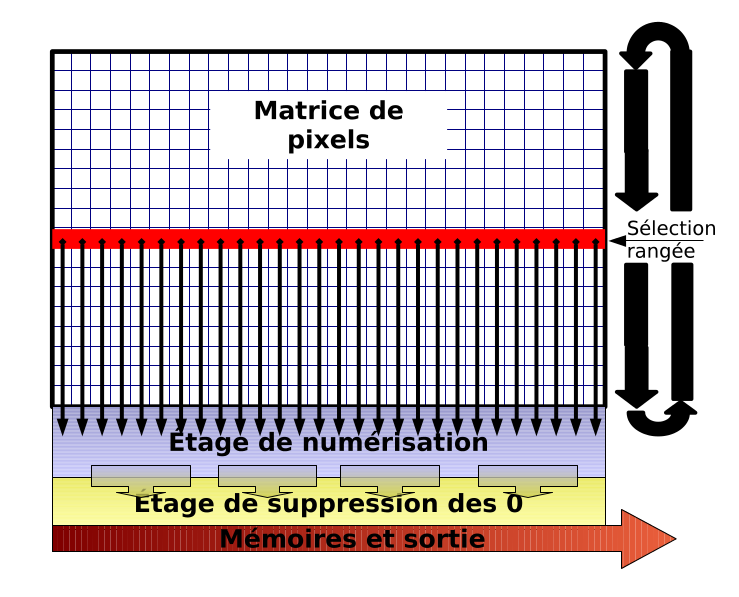
\includegraphics[scale=0.32]{./figures/rolling_shutter.png}
      \caption{Principe de lecture en colonnes parall\`eles}
      \label{fig:rolling_shutter}
    \end{center}
  \end{figure}
   
   \medskip
   
   \renewcommand{\labelitemi}{$\bullet$}
   \begin{itemize}
    \item Discrimination des valeurs des pixels de la ligne N,
    \item Encodage des pixels touch\'es de la ligne N-1,
    \item Lecture de la m\'emoire contenant les positions des pixels touch\'es de la ligne N-2.
   \end{itemize}
  
  \medskip 
   
   Une telle architecture, dite en \textit{volet roulant} de l'anglais \textit{rolling shutter}, permet un temps de lecture \'egal au temps de lecture d'une ligne multipli\'e par le nombre de lignes. Ainsi, pour un capteur de 1000 lignes le temps n\'ecessaire pour la lecture est d'environ 100 $\mu s$. Afin de r\'eduire encore plus le temps de lecture une option consiste \`a r\'ealiser deux sorties, une de chaque côt\'e du capteur. Une autre option dans le cadre d'un d\'etecteur de vertex consiste \`a utiliser des pixels rectangulaires afin de r\'eduire le nombre de lignes en assumant une perte de r\'esolution spatiale selon la direction verticale. Une autre option consiste \`a lire simultan\'ement deux ou quatre lignes pour r\'eduire d'un facteur 2 ou 4 le temps de lecture. Toujours selon le m\^eme principe, une lecture de plusieurs blocs de pixels en parall\`ele pourrait \^etre envisag\'e. On notera aussi que l'on peut obtenir des gains en vitesse de lecture lorsque l'on int\`egre au maximum l'\'electronique de traitement du signal dans les pixels. Le temps de lecture d'une ligne peut ainsi \^etre r\'eduit.
   
   \medskip
   
   Un autre aspect concernant le temps de lecture est le taux d'occupation du capteur. Il s'agit du taux de pixels touch\'es durant la lecture du capteur. L'encodage des pixels touch\'es, la taille de la m\'emoire, et la lecture externe de la m\'emoire limitent le nombre de pixels par ligne pouvant \^etre touch\'es. Le capteur est ainsi optimis\'e pour un taux d'occupation de l'ordre du pour-cents.
  
%    Suppresion de z\'eros
%    Rolling shutter.
%    Pixels rectangulaires
   
   \subsubsection{Puissance dissip\'ee}
   
   La puissance dissip\'ee joue un r\^ole important dans un ensemble instrumental. Pour un d\'etecteur de vertex, celle-ci conditionne le type de refroidissement et donc le budget de mati\`ere. Pour les capteurs d\'eveloppés dans le groupe PICSEL, l'objectif est de fournir des capteurs dont la puissance dissip\'ee est r\'eduite au maximum, afin d'autoriser un refroidissement passif du d\'etecteur de vertex \'etudié. Pour cela, le mode de lecture en volant roulant joue de nouveau un r\^ole majeur. Celui-ci permet en effet de mettre en veille toutes les lignes de pixels sauf celle dont la lecture est en cours. Au final seule une ligne de pixels est allum\'ee. \`A cette ligne de pixels s'ajoute la partie de traitement (lecture, num\'erisation, suppression de z\'eros) \`a l'extr\'emit\'e du capteur. Au total le capteur MIMOSA-26, r\'ealis\'e avec le proc\'ed\'e CMOS 0.35 $\mu m$, consomme 780 $mW$ pour une surface active de 2.2 $cm^2$. En divisant par le nombre de pixels du capteur, on obtient une puissance de 1.1 $\mu W/$pixel. Les capteurs pour l'ILC devront \^etre plus rapide que MIMOSA-26 et consommeront donc plus. L'objectif pour l'ILC est d'obtenir une consommation un ordre de grandeur en dessous de la consommation des pixels hybrides (pixel hybrides : environ 10-30 $\mu W/$pixel). Les d\'etecteurs de l'ILC profiterons du temps mort d'environ 200 $ms$ entre 2 trains de particules pour r\'eduire leurs consommation en passant en veille. C'est ce que l'on appelle le power-pulsing. Ainsi, la consommation des capteurs se voit fortement r\'eduite, ce qui permettra un refroidissement passif du d\'etecteur de vertex.
   
%    Pour le capteur MIMOSA 26, r ́ealis ́e dans la technologie CMOS 0.35 μm, nous obtenons une puissance totale de 780 mW pour 2,2 cm 2 de surface active ou, rapport ́ee au pixel : 1,1μW/pixel.
   
   \subsubsection{Tol\'erance aux radiations}
   
   Nous allons \`a pr\'esent \'etudier la tol\'erance aux radiations des capteurs CMOS d\'eveloppés dans le groupe. Pour cela nous allons distinguer les rayonnements ionisants et les rayonnements non ionisants. Ces deux types de rayonnements agissent de fa\c{c}on diff\'erentes sur les capteurs comme cela a \'et\'e d\'ecrit \`a la section \ref{sect:tolrerance_rad}.
   
   \medskip
   
   Le passage de rayonnements ionisants dans un pixel induit un d\'ep\^ot de charge dans la diode de collection de charges et dans l'\'electronique du pixel. Ces charges s'accumulent et cr\'eent un courant de fuite additionnel. Le fonctionnement du pixel s'en voit perturb\'e et le bruit d\^u aux variations du courant de fuite augmente. Les dégradations li\'ees aux radiations ionisantes d\'ependent de la configuration g\'eom\'etrique de la couche d'oxyde (\'epaisseur et interface) dans laquelle s'accumulent les charges. Afin que les pixels soient moins sensibles aux radiations ionisantes, plusieurs solutions peuvent \^etre envisag\'ees. On peut ainsi optimiser la g\'eom\'etrie des transistors, diminuer l'\'epaisseur des oxydes, diminuer la temp\'erature de fonctionnement du capteur ou encore diminuer le temps d'int\'egration des pixels. L'am\'elioration de la tol\'erance aux radiations est r\'ealisable en utilisant un processus de fabrication dot\'e d'une taille de grille plus fine. Les capteurs CMOS du groupe PICSEL utilisant un processus de fabrication en 0.35 $\mu m$ et dot\'es d'un traitement des donn\'ees simple (donc d'une sortie analogique), r\'esistent \`a une dose ionisante de l'ordre du $MRad$. 
   %Les capteurs \`a sortie binaire, plus rapide et dot\'es d'une sortie plus complexe (plus de transistors) comme MIMOSA-26 et MIMOSA-28 ne r\'esistent qu'à une dose ionisante deux \`a trois fois moindre.
   
   \medskip
   
   Les rayonnements non ionisants provoquent des d\'efauts dans la structure cristalline du silicium et modifie le dopage. Ces d\'efauts deviennent des pi\`eges pour les charges qui d\'erivent dans la couche \'epitaxi\'ee. Le signal s'en voit ainsi diminu\'e. Ainsi, \`a cause des pi\`eges \`a porteurs de charge provoqu\'es par ce type de rayonnements, plus une charge effectue un long parcours dans la couche \'epitaxi\'ee, plus la chance que celle-ci soit pi\'eg\'ee est grande. De ce fait, plus le pas inter-pixels est grand et plus le signal diminue. L'efficacit\'e de d\'etection diminue donc avec la dose de radiations non-ionisantes. Avec une couche \'epitaxi\'ee poss\'edant une r\'esistivit\'e de l'ordre de 50 $\Omega.cm$ et des pixels de 10 $\mu m$ de pas inter-pixels, les capteurs du groupe PICSEL gardent des niveaux de performances identiques jusqu'\`a une fluence \'equivalence d'environ $10^{13} \, n_{eq}.cm^{-2}$. Pour augmenter la r\'esistance \`a ce type de rayonnement, il faut r\'eduire le parcours moyen des porteurs de charge. Pour cela, 2 solutions peuvent \^etre envisag\'ees : la réduction du pas inter-pixels ou l'augmentation de la r\'esistivité de la couche \'epitaxi\'ee. Cette dernière option permet une augmentation de la zone d\'epl\'et\'ee et donc une diminution du libre parcours moyen des porteurs de charge. Enfin, les rayonnements non-ionisants provoquent aussi des d\'efauts cristallins dans les diodes de collection de charges, ce qui induit une augmentation du courant de fuite et par cons\'equent augmente le bruit de grenaille.  
   
%    Les rayonnement non-ionisants agissent selon un m ́ecanisme tr`es diff ́erent. En
% effet, ces derniers cr ́eent des d ́efauts dans le cristal de silicium qui agissent comme
% des pi`eges pour les charges qui constituent le signal et qui d ́erivent dans la zone
% sensible (couche  ́epitaxi ́ee). Il faut rappeler (voir paragraphe 3.2.1) que les charges
% d ́erivent thermiquement car la technologie standard des capteurs `a pixels CMOS
% ne permet pas d’appliquer un potentiel  ́elev ́e (quelques dizaines de volts) de part
% et d’autre de la couche  ́epitaxi ́ee afin de g ́en ́erer un champ de d ́erive. L’effet de la
% radiation non-ionisante sera donc de diminuer le signal de mani`ere d’autant plus
% importante que la distance entre les diodes de collection est grande (c’est `a dire
% que la taille des pixels est grande).
% Avec une couche pr ́esentant une r ́esistivit ́e de l’ordre de 50 Ω.cm et des
% pixels de10 μm de pas, les capteurs de la s ́erie MIMOSA ont montr ́e qu’ils
% conservaient leurs performances nominales jusque vers une fluence  ́equivalente
% `a 10 13 neq ·cm −2 . L’am ́elioration de cette tol ́erance requiert l’utilisation d’une
% couche  ́epitaxi ́ee de r ́esistivit ́e plus  ́elev ́ee de l’ordre du kΩ. Les tests de proto-
% types b ́en ́eficiant de cette couche sensible ont effectivement montr ́e qu’un gain
% d’un ordre de grandeur pouvait ˆetre esp ́er ́e [Dor10].
   
%    \section{Acquisition et lecture des donn\'ees}
   
   \subsection{Performances}
   
   Depuis une quinzaine d'ann\'ees une trentaine de prototypes de capteurs CMOS MIMOSA ont \'et\'e d\'evelopp\'es et test\'es. Ainsi, au cours de ces ann\'ees les performances de ces capteurs CMOS pour la physique des hautes \'energies ont pu \^etre caract\'eris\'ees. Diff\'erents prototypes de capteurs CMOS con\c{c}us \`a partir de diff\'erents proc\'ed\'es de gravure, de diff\'erents pas inter-pixels et de diff\'erentes \'epaisseurs de couche \'epitaxi\'ee ont vu le jour. Ces capteurs ont \'et\'e test\'es en laboratoire et en faisceaux. Ces tests ont aussi \'et\'e r\'ealis\'es pour diff\'erentes temp\'eratures et diff\'erents niveaux d'irradiations. Nous allons en pr\'esenter les performances g\'en\'erales obtenues.
  
   \medskip
   
  \begin{figure}[!htb]
   \begin{center}
     \subfigure[Efficacit\'e de d\'etection en fonction du taux d'impact fant\^omes pour le capteur MIMOSA-9.]{
      \label{fig:eff_fhr}
      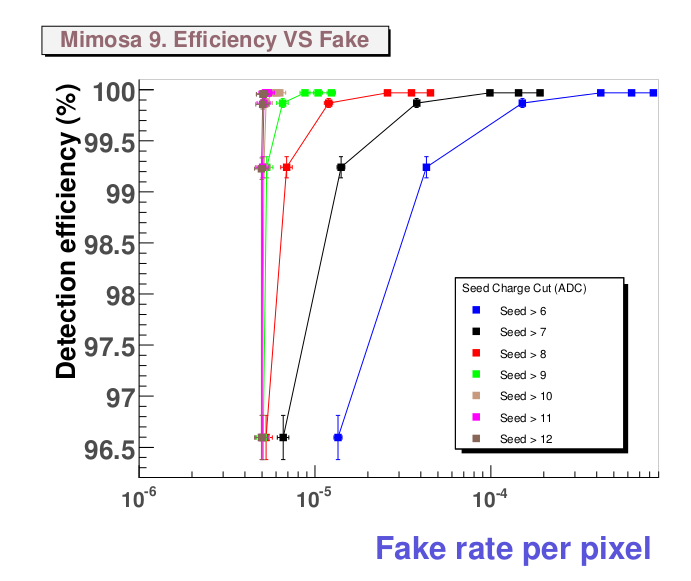
\includegraphics[width=0.47\textwidth]{./figures/eff_fake_hit_rate.png}
     }
     \subfigure[R\'esolution spatiale en fonction du pas inter-pixel (pitch) pour les diff\'erents capteurs MIMOSA.]{
      \label{fig:reso_pitch}
      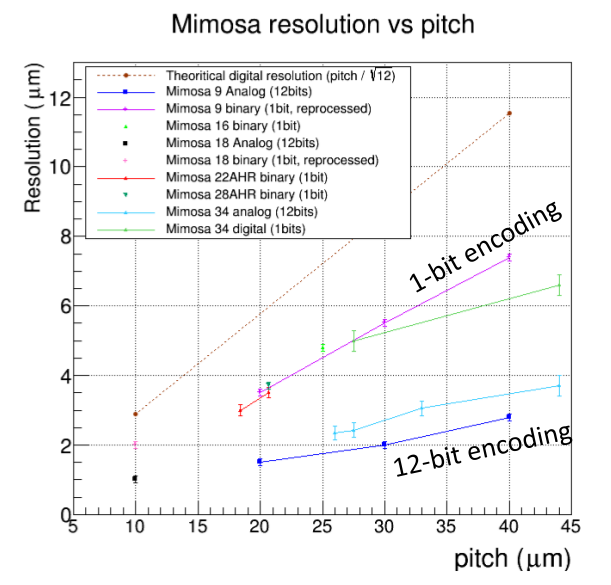
\includegraphics[width=0.47\textwidth]{./figures/reso_vs_pitch.png}
     }
   \caption{Performances des capteurs CMOS d\'eveloppés dans le groupe.}
   \label{fig:Ultimate}
   \end{center}
  \end{figure}
  
%   \begin{figure}[!htb]
%     \begin{center} 
%       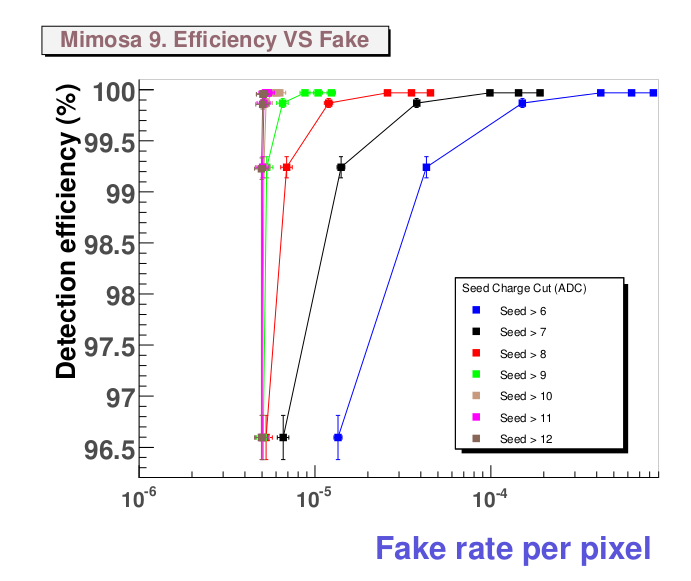
\includegraphics[scale=0.35]{./figures/eff_fake_hit_rate.png}
%       \caption{Efficacit\'e de d\'etection en fonction du taux d'impact fant\^omes pour le capteur MIMOSA-9.}
%       \label{fig:eff_fhr}
%     \end{center}
%   \end{figure} 
%    
%    \begin{figure}[!htb]
%     \begin{center} 
%       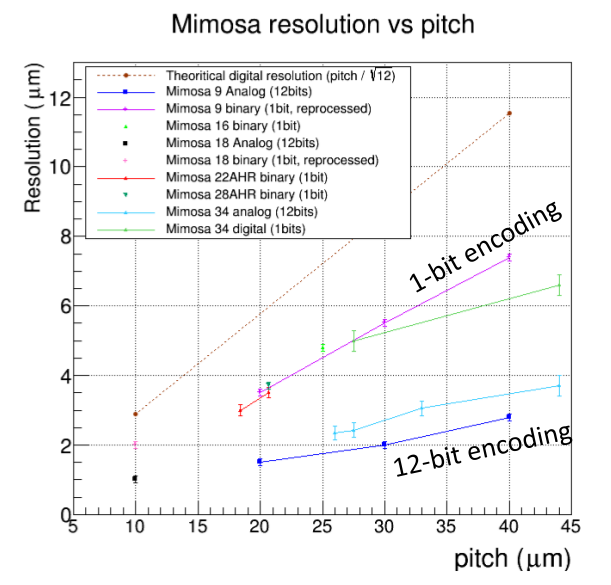
\includegraphics[scale=0.45]{./figures/reso_vs_pitch.png}
%       \caption{R\'esolution spatiale en fonction du pas inter-pixel (pitch) pour les diff\'erents capteurs MIMOSA.}
%       \label{fig:reso_pitch}
%     \end{center}
%   \end{figure}
   
   Les capteurs \`a sortie analogique permettent de lire directement le signal collect\'e dans chaque pixel et d'en mesurer le bruit. Ainsi, selon l'\'epaisseur de la couche \'epitaxi\'ee et la r\'epartition des charges, la charge collect\'ee dans le pixel si\`ege varie. Toutefois celle-ci est de l'ordre de quelques centaines d'\'electrons collect\'es (200-300 $e^-$). Le bruit mesur\'e avoisine quant \`a lui la dizaine d'\'electrons \`a 20\textcelsius $\,$ et le signal sur bruit ainsi obtenu est de l'ordre de 20 \`a 40. Cela correspond \`a une efficacit\'e  de d\'etection d'environ 100 $\%$ pour un taux d'impacts fant\^omes sous la barre des $10^{-4}$. Ces performances sont visibles pour le capteur MIMOSA-9 en figure \ref{fig:eff_fhr}  
  
  \medskip
   
   La r\'esolution spatiale d\'epend du pas inter-pixel et du type de sortie : analogique ou binaire du capteur. Pour des capteurs \`a sortie analogique, la r\'esolution spatiale varie quasi-lin\'eairement entre une valeur inf\'erieure ou \'egale au microm\`etre pour un pas inter-pixel de 10 $\mu m$ et une valeur d'environ 3 $\mu m$ pour un pas inter-pixel de 40 $\mu m$. Ces valeurs sont atteintes avec l'algorithme de la fonction $\eta$ pr\'esent\'e en section \ref{sect:reso}. Pour un capteur \`a sortie binaire, une r\'esolution spatiale de l'ordre de 3 microm\`etres est atteinte pour un pas inter-pixel de 15 $\mu m$. Ces r\'esultats sont visibles en figure \ref{fig:reso_pitch}.
   
   \medskip
   
   Comme nous l'avons vu, les radiations ionisantes conduisent \`a l'accumulation de charges dans les interfaces, ce qui entraîne une augmentation du bruit des pixels. Les performances des capteurs peuvent \^etre maintenues acceptables avec une irradiation d'environ 1 $MRad$ et un refroidissement mod\'er\'e. Un passage \`a un proc\'ed\'e de fabrication utilisant une taille de grille plus fine permet l'am\'elioration de cette tol\'erance aux radiations grâce notamment \`a la r\'eduction de la couche d'oxyde \cite{Deveaux:2011}. Les radiations non ionisantes sont fortement d\'ependantes de la taille du pas inter-pixel. Les capteurs avec un pas inter-pixel de 10 $\mu m$ r\'esistent \`a un flux de $10^{13} n_{eq}/cm^2$ alors que ceux dot\'es d'un pas inter-pixel de 20 $\mu m$ ne r\'esistent qu'a une fluence de $2 \times 10^{12} n_{eq}/cm^2$. L'am\'elioration de cette tol\'erance n\'ecessite l'utilisation de couche \'epitaxi\'ee de plus haute r\'esistivit\'e, de l'ordre du $k \Omega$. Les tests de tels capteurs ont montr\'e un gain d'un ordre de grandeur \cite{Dorokhov2010432}.
   
%  MIMOSA 28
%  con\c{c}u pour STAR

  \FloatBarrier
   
   \subsection{ULTIMATE : MIMOSA-28}
   \label{sub:MIMOSA28}
   
   L'\'etat de l'art des capteurs CMOS pour la physique des particules est repr\'esent\'e par le capteur MIMOSA-28 alias ULTIMATE \cite{1748-0221-7-01-C01102}. Ce capteur est illustr\'e en figure \ref{fig:Ultimate}. Il s'agit du premier capteur \`a \^etre int\'egr\'e dans une exp\'erience de physique des particules, \`a savoir STAR \`a RHIC. Ce capteur constitue la derni\`ere \'etape dans le développement d'un capteur pour \'equiper les deux premi\`eres couches (STAR-PXL) du d\'etecteur de vertex de l'exp\'erience STAR : le Heavy Flavour Tracker (HFT).

  \begin{figure}[!htb]
   \begin{center}
     \subfigure[Sch\'ema de MIMOSA-28.]{
      \label{fig:ultimate_schema}
      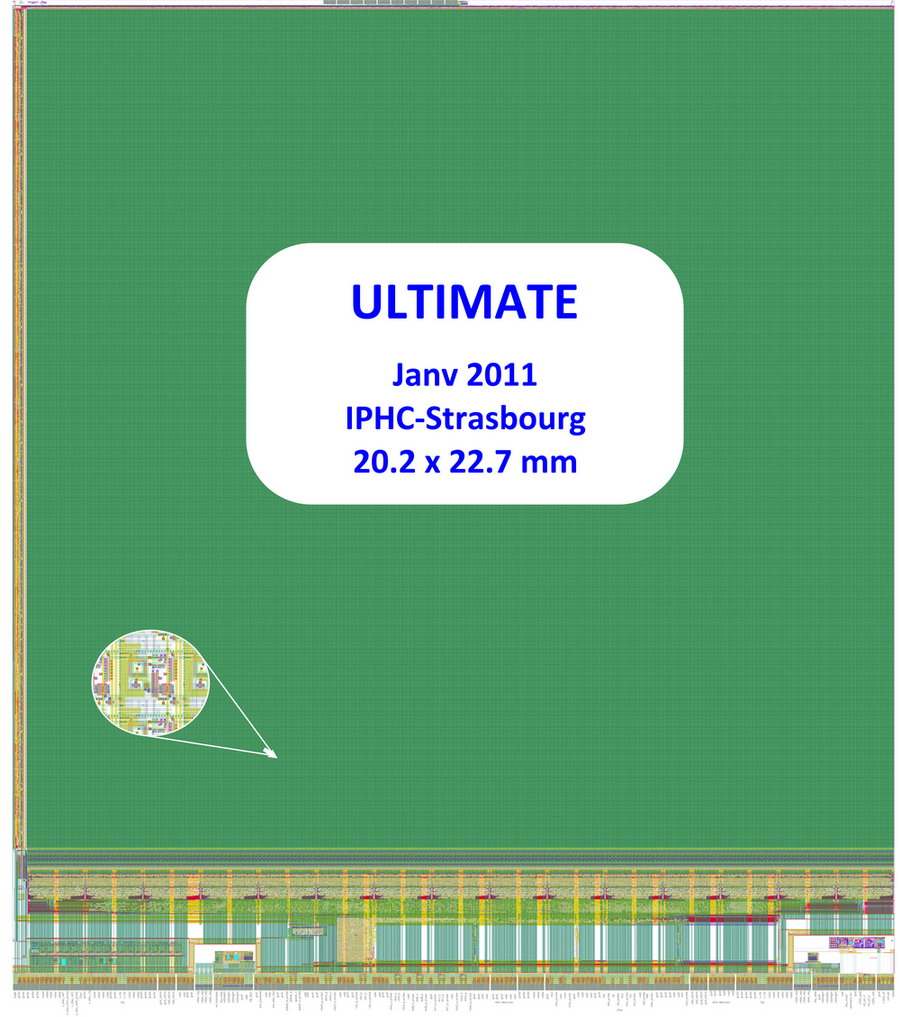
\includegraphics[width=0.32\textwidth]{./figures/Ultimate_small.jpg}
     }
     \subfigure[Photo d'un capteur MIMOSA-28.]{
      \label{fig:ultimate_photo}
      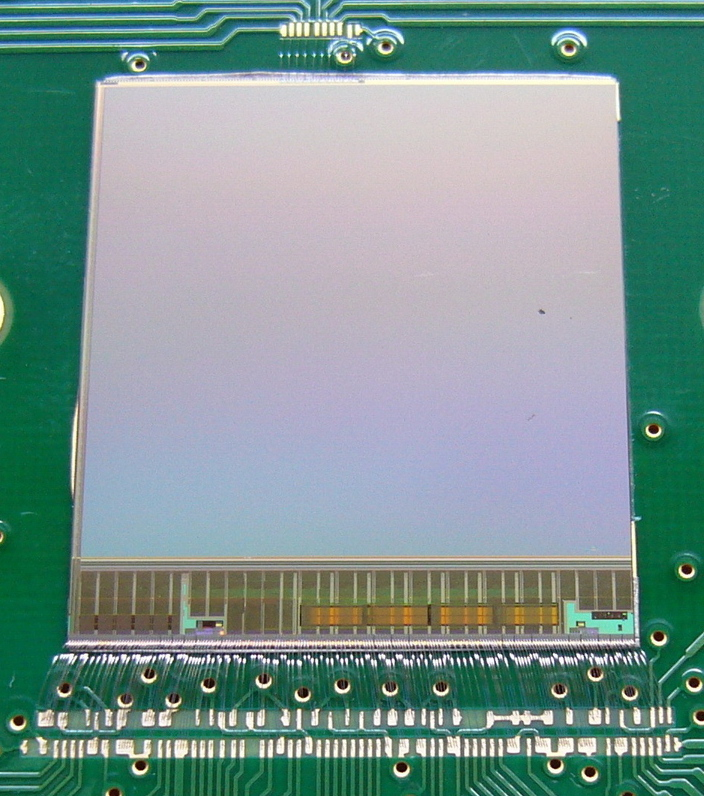
\includegraphics[width=0.32\textwidth]{./figures/ultimate_photo.jpg}
     }
   \caption{Repr\'esentation du capteur MIMOSA-28 alias ULTIMATE.}
   \label{fig:Ultimate}
   \end{center}
  \end{figure}

   \medskip
  
   ULTIMATE est compos\'e d'une matrice de 928 (lignes) $\times$ 960 (colonnes) pixels et est dot\'e d'un pas inter-pixel de 20.7 $\mu m$. Le capteur mesure 20.22 mm $\times$ 22.71 $mm^2$ et est confectionn\'e \`a partir du processus de gravure AMS 0.35 $\mu m$. Il est dot\'e d'une sortie binaire (plus une sortie secondaire analogique beaucoup plus lente r\'eserv\'ee aux tests en laboratoire) et d'un circuit de suppression de z\'ero. La lecture des pixels s'effectue gr\^ace \`a l'architecture en volet roulant et la dur\'ee d'int\'egration est inf\'erieure \`a 200 $\mu s$. Le capteur est con\c{c}u pour une tenue aux radiations de 150 $kRad$ de dose ionisante et une fluence de $3 \times 10^{12} n_{eq}/cm^2$ \`a sa temp\'erature de fonctionnement de 35 \textcelsius. Côt\'e budget de mati\`ere, ce capteur peut \^etre aminci \`a une \'epaisseur de 50 $\mu m$, 
  
     % avant figure = mi28_epi20_caract.png
   
  \begin{figure}[!htb]
    \begin{center}
      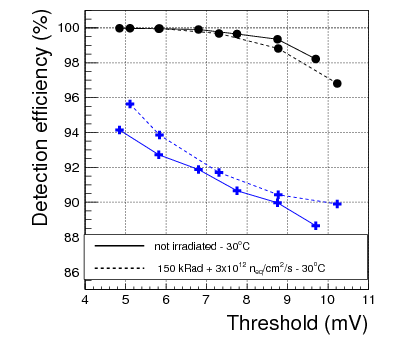
\includegraphics[scale=0.55]{./figures/m28_3colorsPlot_compareIrrad_BW.png}
      \caption{Efficacit\'e et taux d'impacts fant\^omes pour le capteur MIMOSA-28 \cite{Baudot:2013pc}.}
      \label{fig:caract_mi28_20}
    \end{center}
  \end{figure}
  
  \medskip
  
   Côt\'e performances, ULTIMATE offre une efficacit\'e d'environ 100 $\%$ pour un taux d'impacts fant\^omes inf\'erieur \`a $10^{-5}$ et permet une r\'esolution spatiale inf\'erieure \`a 4 $\mu m$. La figure \ref{fig:caract_mi28_20} illustre l'efficacit\'e et le taux d'impacts fant\^omes en fonction du seuil des discriminateurs, le tout pour diff\'erents types d'irradiations.
  
  \medskip
  
   \textit{ULTIMATE}, \'equipe depuis fin 2013 le premier d\'etecteur de vertex bas\'e sur les capteurs \`a pixels CMOS. Nomm\'e \textit{STAR-PXL}, ce d\'etecteur de vertex est confectionn\'e \`a partir de deux couches cylindriques, de rayon $2.5$ et $8$ $cm$. Il est constitu\'e de 40 \'echelles comportant chacune 10 capteurs MIMOSA-28, soit d'environ 370 $MPixels$. Le budget de mati\`ere pour chaque \'echelle s'\'el\`eve \`a $0.37\% \, X0$.
   
%    General description of STAR CMOS pixel sensor
% Ultimate is the final sensor chip for the upgrade of STAR inner layer of the vertex detector. Its
% architecture integrates main function of Mimosa26 (Monolithic Active Pixel Sensor (MAPS) with fast
% binary readout) and including a zero suppression logic. The sensor consists of a matrix composed by
% 928 (rows) x 960 (columns) pixels of 20.7 μm pitch for a size of the chip of 20.22 mm x 22.71 mm.
% The design process Austria Micro System AMS-C35B4/OPTO uses 4 metal- and 2 poly- layers. The
% thickness of the epitaxial layer stretches out up to 15 μm in Hi-Resistivity substrate (400 Ohm.cm).
% The design tools follow the CADENCE DFII 5.1 with DIVA, ASSURA, CALIBRE rules. The
% chip has been submitted in an Engineering Run via CMP on 20 January 2011
% In the STAR vertex detector, the hit rate is evaluated at 2.4 x 10 5 hits/s/cm2. The design of the
% sensor is driven by the high readout frequency in order to keep the track multiplicity per frame at a low
% level. It is done by read out pixel columns in parallel, row by row. The chip readout time is 185.6 μs.
% Each pixel includes an amplification and Correlated Double Sampling (CDS) and each end of column
% is equipped with a discriminator. The threshold of the discriminator is programmable by slow control.
% After analogue to digital conversion, digital signals pass through the zero suppression block. The
% digital signals are processed in parallel on 15 banks, then arranged and stored in a memory row by
% row. Two memories banks have been implemented in the sensor to perform read and write operations
% simultaneously (see §Memory management).
% At each frame, the circuit sends a specific marker to initialize the formatted readout and inside the
% data, some specifics words give also synchronization markers to begin and start the readout.
% The chip offers the choice of the output bit rate of the communication. 160 or 80 Mbits /second.
   
   
%    Mimosa 28.
   
  %Comment ca fonctionne \\
  %les differentes couches et dopages \\
  %diffusion des electron et captage par les puits N. \\
  %architecture du pixel \\
  %Schemas de fonctionnement \\
  %Partie DAQ. (Aller voir Matthieu et Gilles) \\
  
  \subsection{Conclusion}
  
  Dans cette section nous avons vu que les capteurs CMOS sont de bons candidats pour les d\'etecteurs de vertex du futur et en particulier pour celui de l'ILD. Ils offrent en effet, une tr\`es bonne r\'esolution spatiale pour un budget de mati\`ere r\'eduit. De plus les nombreux développements ax\'es sur la vitesse de lecture, la tenue aux radiations et la puissance dissip\'ee permettent de proposer des capteurs CMOS r\'epondant aux exigences du cahier des charges du détecteur de vertex de l'ILD. L'int\'egration de ces capteurs constitue une \'etape de plus vers la r\'ealisation d'un tel d\'etecteur. Afin de tester les capteurs CMOS du futur et l'int\'egration de ces capteurs CMOS, un télescope en faisceau de grande pr\'ecision et de grande surface est requis. Ce télescope devra voir le jour sous l'\'egide du projet europ\'een AIDA (Advanced European Infrastructure for detectors at Accelerators).
  
  %   \section{Comparaison des technologies}

  
\section{AIDA : Advanced European Infrastructure for detectors at Accelerators}

  Comme nous l'avons vu le d\'etecteur de vertex pour l'ILD demande une pr\'ecision sur le param\`etre d'impact encore in\'egal\'ee. Pour \'evaluer et d\'evelopper les performances des prototypes de capteurs pix\'elis\'es pour l'ILD, un télescope de grande surface dot\'e d'une grande pr\'ecision permettra de r\'ealiser des tests en faisceau d'un secteur de d\'etecteur de vertex. Fort du succ\`es du télescope EUDET, le projet AIDA s'enrichira d'un nouveau télescope en faisceau qui permettra un nouveau pas vers la r\'ealisation des détecteurs du futur.

\subsection{Work Package 9.3 : Precision Pixel Detector Infrastructure}

 Afin d'\'evaluer les performances et dans le but de développer les d\'etecteurs de particules de demain, des tests en faisceaux de ceux-ci sont n\'ecessaires. Pour les d\'etecteurs participant \`a la trajectom\'etrie, il faut pouvoir identifier des traces dans le but de tester les param\`etres des d\'etecteurs comme leur r\'esolution spatiale ou leur efficacit\'e de d\'etection. Pour cela les télescopes en faisceau constituent des outils adapt\'es. Depuis plusieurs ann\'ees, diff\'erents t\'elescopes ont \'et\'e construits.

 \medskip

 Le télescope en faisceau \textit{EUDET} \cite{behr2010test} a \'et\'e propos\'e afin de disposer d'un t\'elescope en faisceau standardis\'e et polyvalent. Ce télescope de grande pr\'ecision bas\'e sur des capteurs pix\'elis\'es a \'et\'e con\c{c}u pour accueillir et tester diff\'erents type de capteurs. Le syst\`eme d'acquisition standardis\'e propos\'e permet une mise en route rapide des tests. En vertu de son budget de mati\`ere r\'eduit, le télescope \textit{EUDET} peut \^etre utilis\'e avec des particules de faibles impulsions (quelques centaines de $MeV$). Ce t\'elescope est compos\'e de 6 plans MIMOSA-26 amincis \`a 50 $\mu m$. Chaque capteur MIMOSA-26 est compos\'e de 1152 $\times$ 576 pixels espac\'es d'un pas inter-pixels de 18.4 $\mu m$ repr\'esentant une surface active de $21.2 \times 10.6 \, mm^2$. Chacun des plans offre ainsi une r\'esolution spatiale de $4 \, \mu m$. Le t\'elescope offre un syst\`eme de positionnement pr\'ecis des plans qui le constituent. Ce syst\`eme permet d'effectuer des translations et une rotation du capteur test\'e afin d'en explorer les propri\'et\'es sur l'ensemble de sa surface. La m\'ecanique du t\'elescope a de plus \'et\'e con\c{c}ue de fa\c{c}on à fournir un t\'elescope transportable. Au SPS, avec un faisceau de pions charg\'es d'une impulsion de 120 $GeV/c$, ce t\'elescope fournit une r\'esolution extrapol\'ee minimale meilleure que 2 $\mu m$. Les capteurs test\'es de grandes tailles peuvent de plus \^etre plac\'es en bout de t\'elescope en assumant une r\'esolution extrapol\'ee moins bonne. Une plate-forme logicielle pour le syst\`eme d'acquisition nomm\'ee \textit{EUDAQ} autorise l'int\'egration du capteur test\'e et de son syst\`eme d'acquisition dans le flux de donn\'ees du télescope.

 %(25 $\mu m$ \`a 1.5 $m$ du dernier plan par exemple)
 
   \begin{figure}[!htb]
    \begin{center} 
      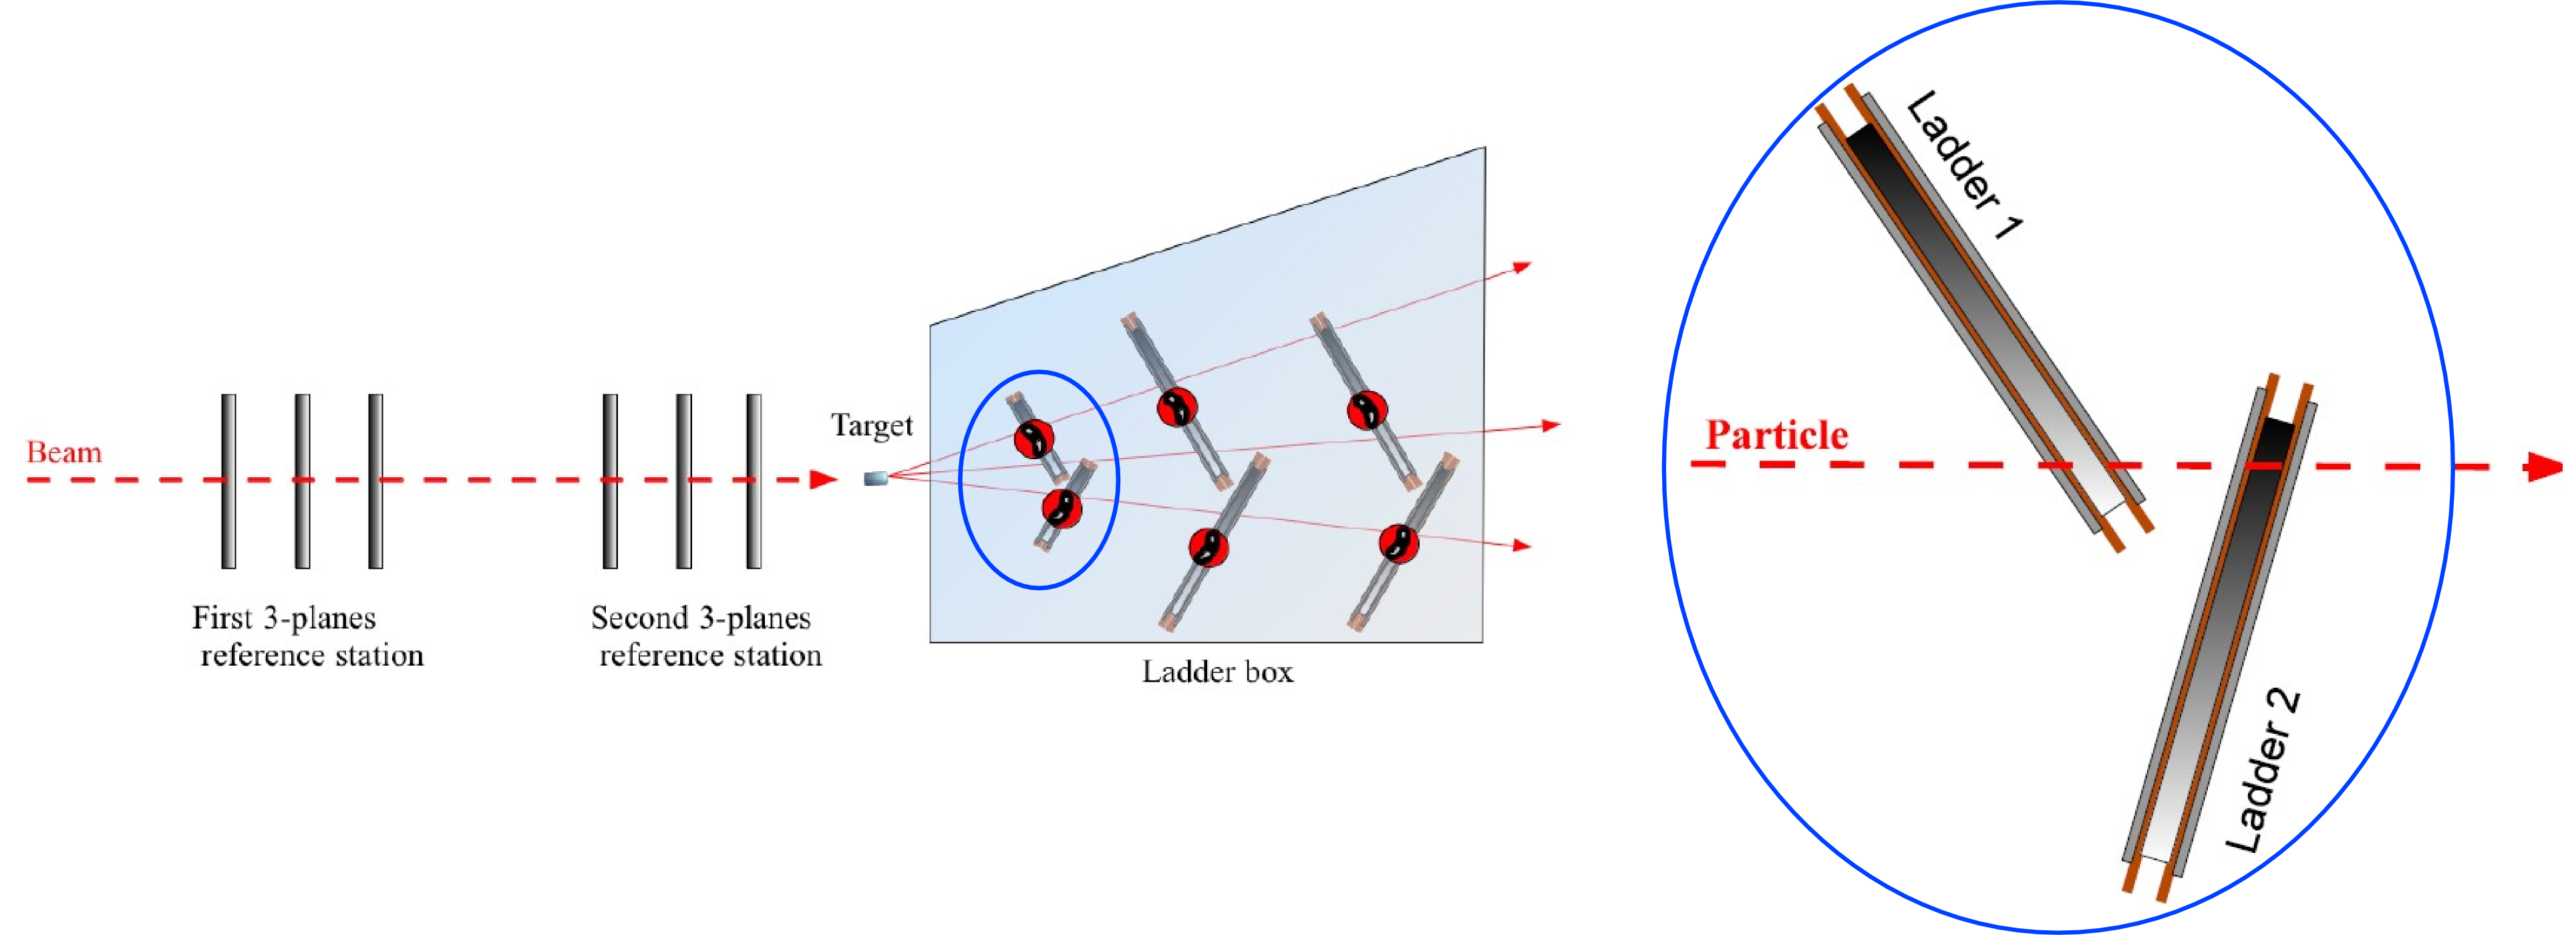
\includegraphics[scale=0.30]{./figures/AIDA_telescope.png}
      \caption{Telescope en faisceau AIDA}
      \label{fig:AIDA_tel}
    \end{center}
  \end{figure}
 
 \medskip

 Le t\'elescope en faisceau \textit{AIDA}, dans la lign\'e du télescope \textit{EUDET}, constituera un t\'elescope d\'evou\'e aux d\'eveloppements des futurs trajectom\`etres. Ce télescope en faisceau permettra ainsi le développement des d\'etecteurs du syst\`eme de trajectom\'etrie pour l'ILC ou encore pour sLHC. Ce t\'elescope illustr\'e en figure \ref{fig:AIDA_tel} sera muni d'un bras de télescope, d'une cible et d'un secteur de d\'etecteur de vertex nomm\'e \textit{boîte AID} (\textit{Alignment Investigation Device}). Afin de r\'epondre aux diff\'erents besoins, le bras de télescope sera interchangeable, et plusieurs capteurs de technologies diff\'erentes pourront l'\'equiper. Le choix de la technologie pour ce premier bras de t\'elescope sera fait selon les besoins de l'utilisateur. Les pixels hybrides utilis\'es par l'exp\'erience ATLAS nomm\'es \textit{FE-I4} permettront une vitesse de lecture équivalente \`a celle du LHC (de l'ordre de 25 $ns$), les capteurs \textit{TimePix} permettront un \'etiquetage temporel encore meilleur ($\approx$ 10 $ns$) avec une bonne r\'esolution spatiale, enfin les super-plans \textit{SALAT} d\'eveloppés dans le groupe \textit{PICSEL} offriront une grande surface ($4 \times 4 \, cm^2$), une r\'esolution spatiale accrue de l'ordre de $3.5 \, \mu m$, pour un temps de lecture d'environ 200 $\mu s$ et un budget de mati\`ere r\'eduit (capteurs amincis \`a 50 $\mu m$).

% Task 9.3: Precision Pixel Detector Infrastructure
% 
% Silicon pixel detectors are used in the inner most layers of particle detectors. Development of detectors with extremely high precision is taking place in future collider experiment projects. To evaluate the performance of these silicon pixel detector prototypes, a reference device with high precision (a telescope) is needed. Based on the success of the telescope built with EUDET, this task will built a new telescope fulfilling both the requirements in term of high precision (as needed by the Linear Collider prototypes) and in term of read-out speed (as required by the SLHC community). Silicon detectors need to operate in well controlled low temperature and humidity environment, and their position should be known and monitored accurately. The telescope built under this task is expected to be used as a test bench for a new cooling system and for thermo-mechanical devices and thermal imaging techniques which will be used to monitor minute misalignments and deformations.

  \subsection{SALAT}

  SALAT est un télescope conçu par le groupe \textit{PICSEL} pour constituer le premier bras du télescope \textit{AIDA}. Il croisera ainsi le faisceau en premier. SALAT sera compos\'e de 3 super-plans de grande surface et de grande pr\'ecision. Cette grande surface est n\'ecessaire pour fournir une reconstruction des traces issues d'un large faisceau afin de pouvoir fournir une large zone d'impact sur la cible ou sur la boîte \textit{AID}. Les impacts sur la cible provoqueront des vertex qui se repartiront notamment sur la boite \textit{AID}. Ainsi, la boite \textit{AID} pourra \^etre couverte. 
  
  \medskip
  
  Chacun des trois super-plans \textit{SALAT} poss\`edent une zone sensible mesurant $4 \times 3.8 \, cm^2$ et une r\'esolution spatiale de l'ordre de $3.5 \, \mu m$. Chaque super-plan est lui m\^eme compos\'e de 4 capteurs MIMOSA-28 (voir section \ref{sub:MIMOSA28}). Le temps de lecture de chaque super-plan est ainsi équivalent \`a celui de MIMOSA-28, et vaut environ $200 \, \mu s$. Les 4 capteurs d'un super-plan sont coll\'es sur une feuille de Mylar pr\'ealablement tendue (plus grande rigidit\'e) d'une \'epaisseur d'environ $50 \, \mu m$. Le super-plan poss\`ede ainsi une longueur de radiation de $X0 = 28.7 \, cm$ (environ 3 fois celle du silicium).
  
  \begin{figure}[!htb]
    \begin{center} 
      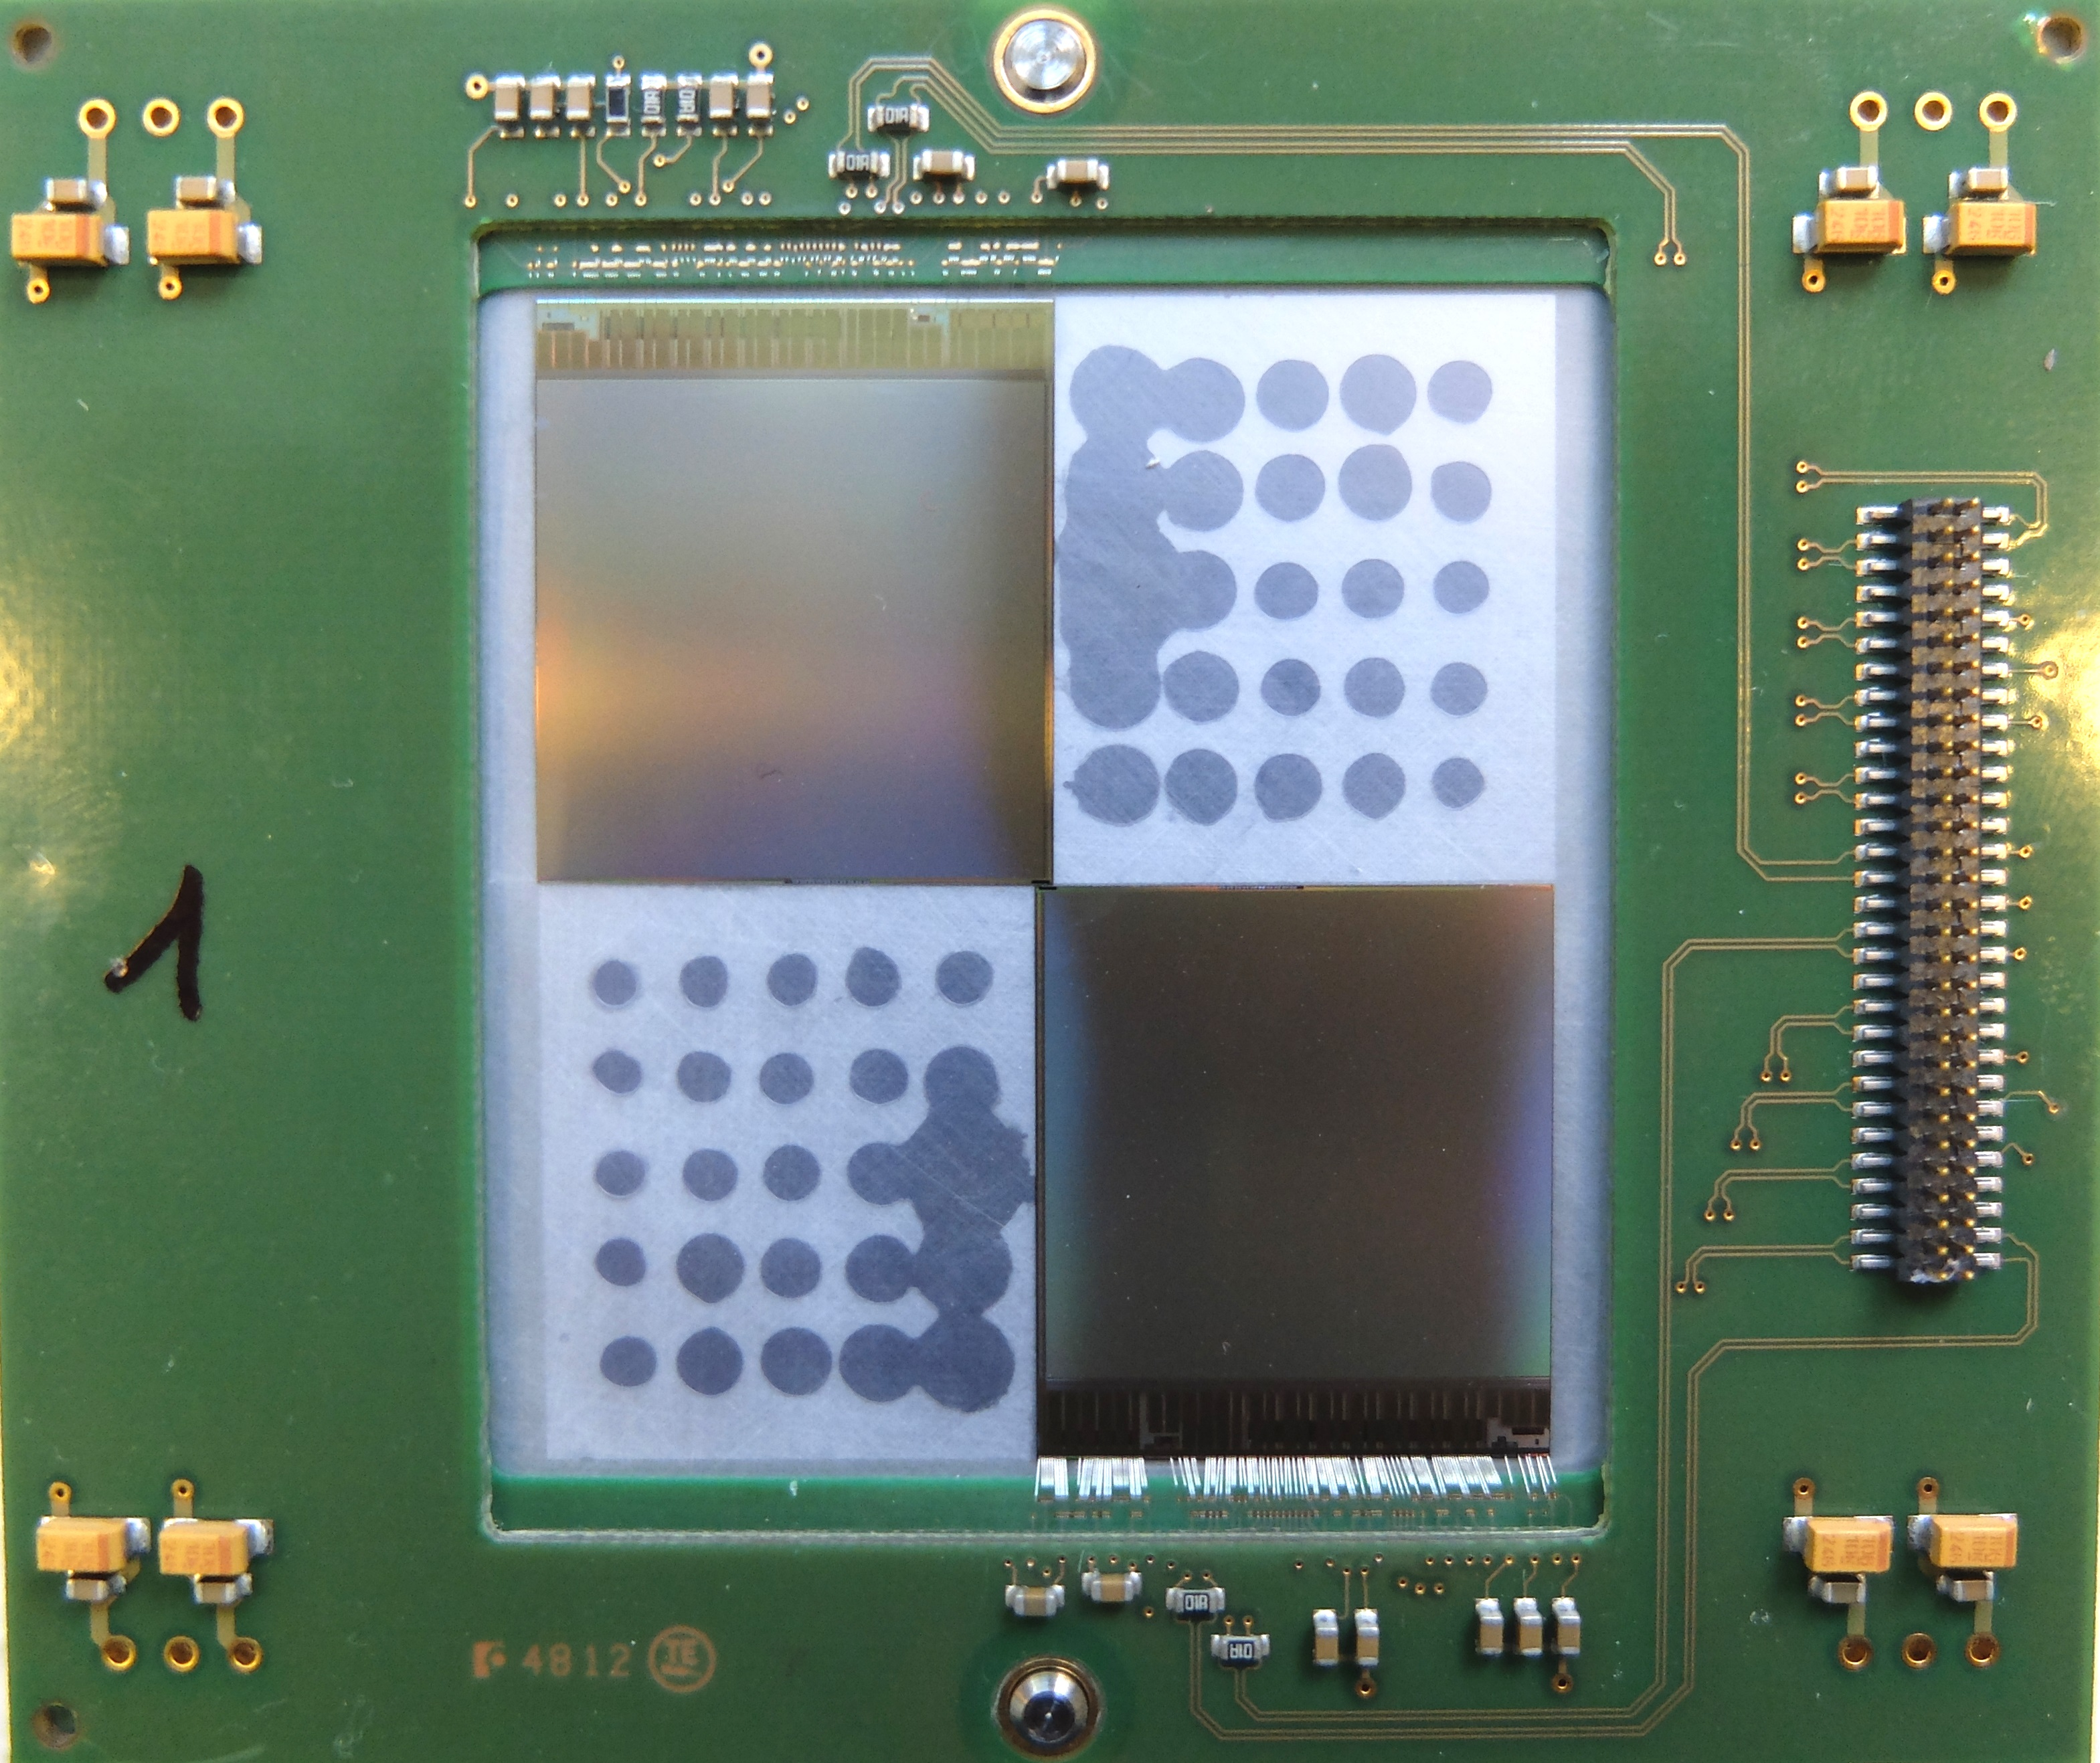
\includegraphics[scale=0.07]{./figures/SALAT_2.jpg}
      \caption{SALAT – Single Arm Large Area beam Telescope}
      \label{fig:SALAT}
    \end{center}
  \end{figure}

   \medskip
  
  Nous allons num\'eroter les capteurs de 1 \`a 4. La face avant du super-plan est d\'efinie par la figure \ref{fig:coordCapteurSALAT00}. C'est cette face qui sera touch\'ee en premier par le faisceau lors des tests en faisceau. Si l'on prend un axe $Oz$ perpendiculaire au super-plan et passant en son centre au point $O$ d\'efini au milieu de la feuille de Mylar, la face avant du super-plan est d\'efinie par des coordonn\'ees $z$ n\'egatives et la face arri\`ere par des coordonn\'ees $z$ positives. Les capteurs num\'erot\'es 1 et 4 sont alors situ\'es sur la face avant ($z$ n\'egatifs) du super-plan. Sur cette face, le capteur 1 se situe en bas \`a gauche et le capteur 4 est plac\'e en haut \`a droite. Les capteurs 2 et 3 sont coll\'es \`a la face arri\`ere du super-plan ($z$ positifs). Le capteur 2 se situe en bas \`a droite alors que le capteur 3 se situe en haut \`a gauche lorsque l'on regarde le super-plan par la face avant (voir figure \ref{fig:coordCapteurSALAT00}).
    
   \begin{figure}[!htb]
    \begin{center} 
      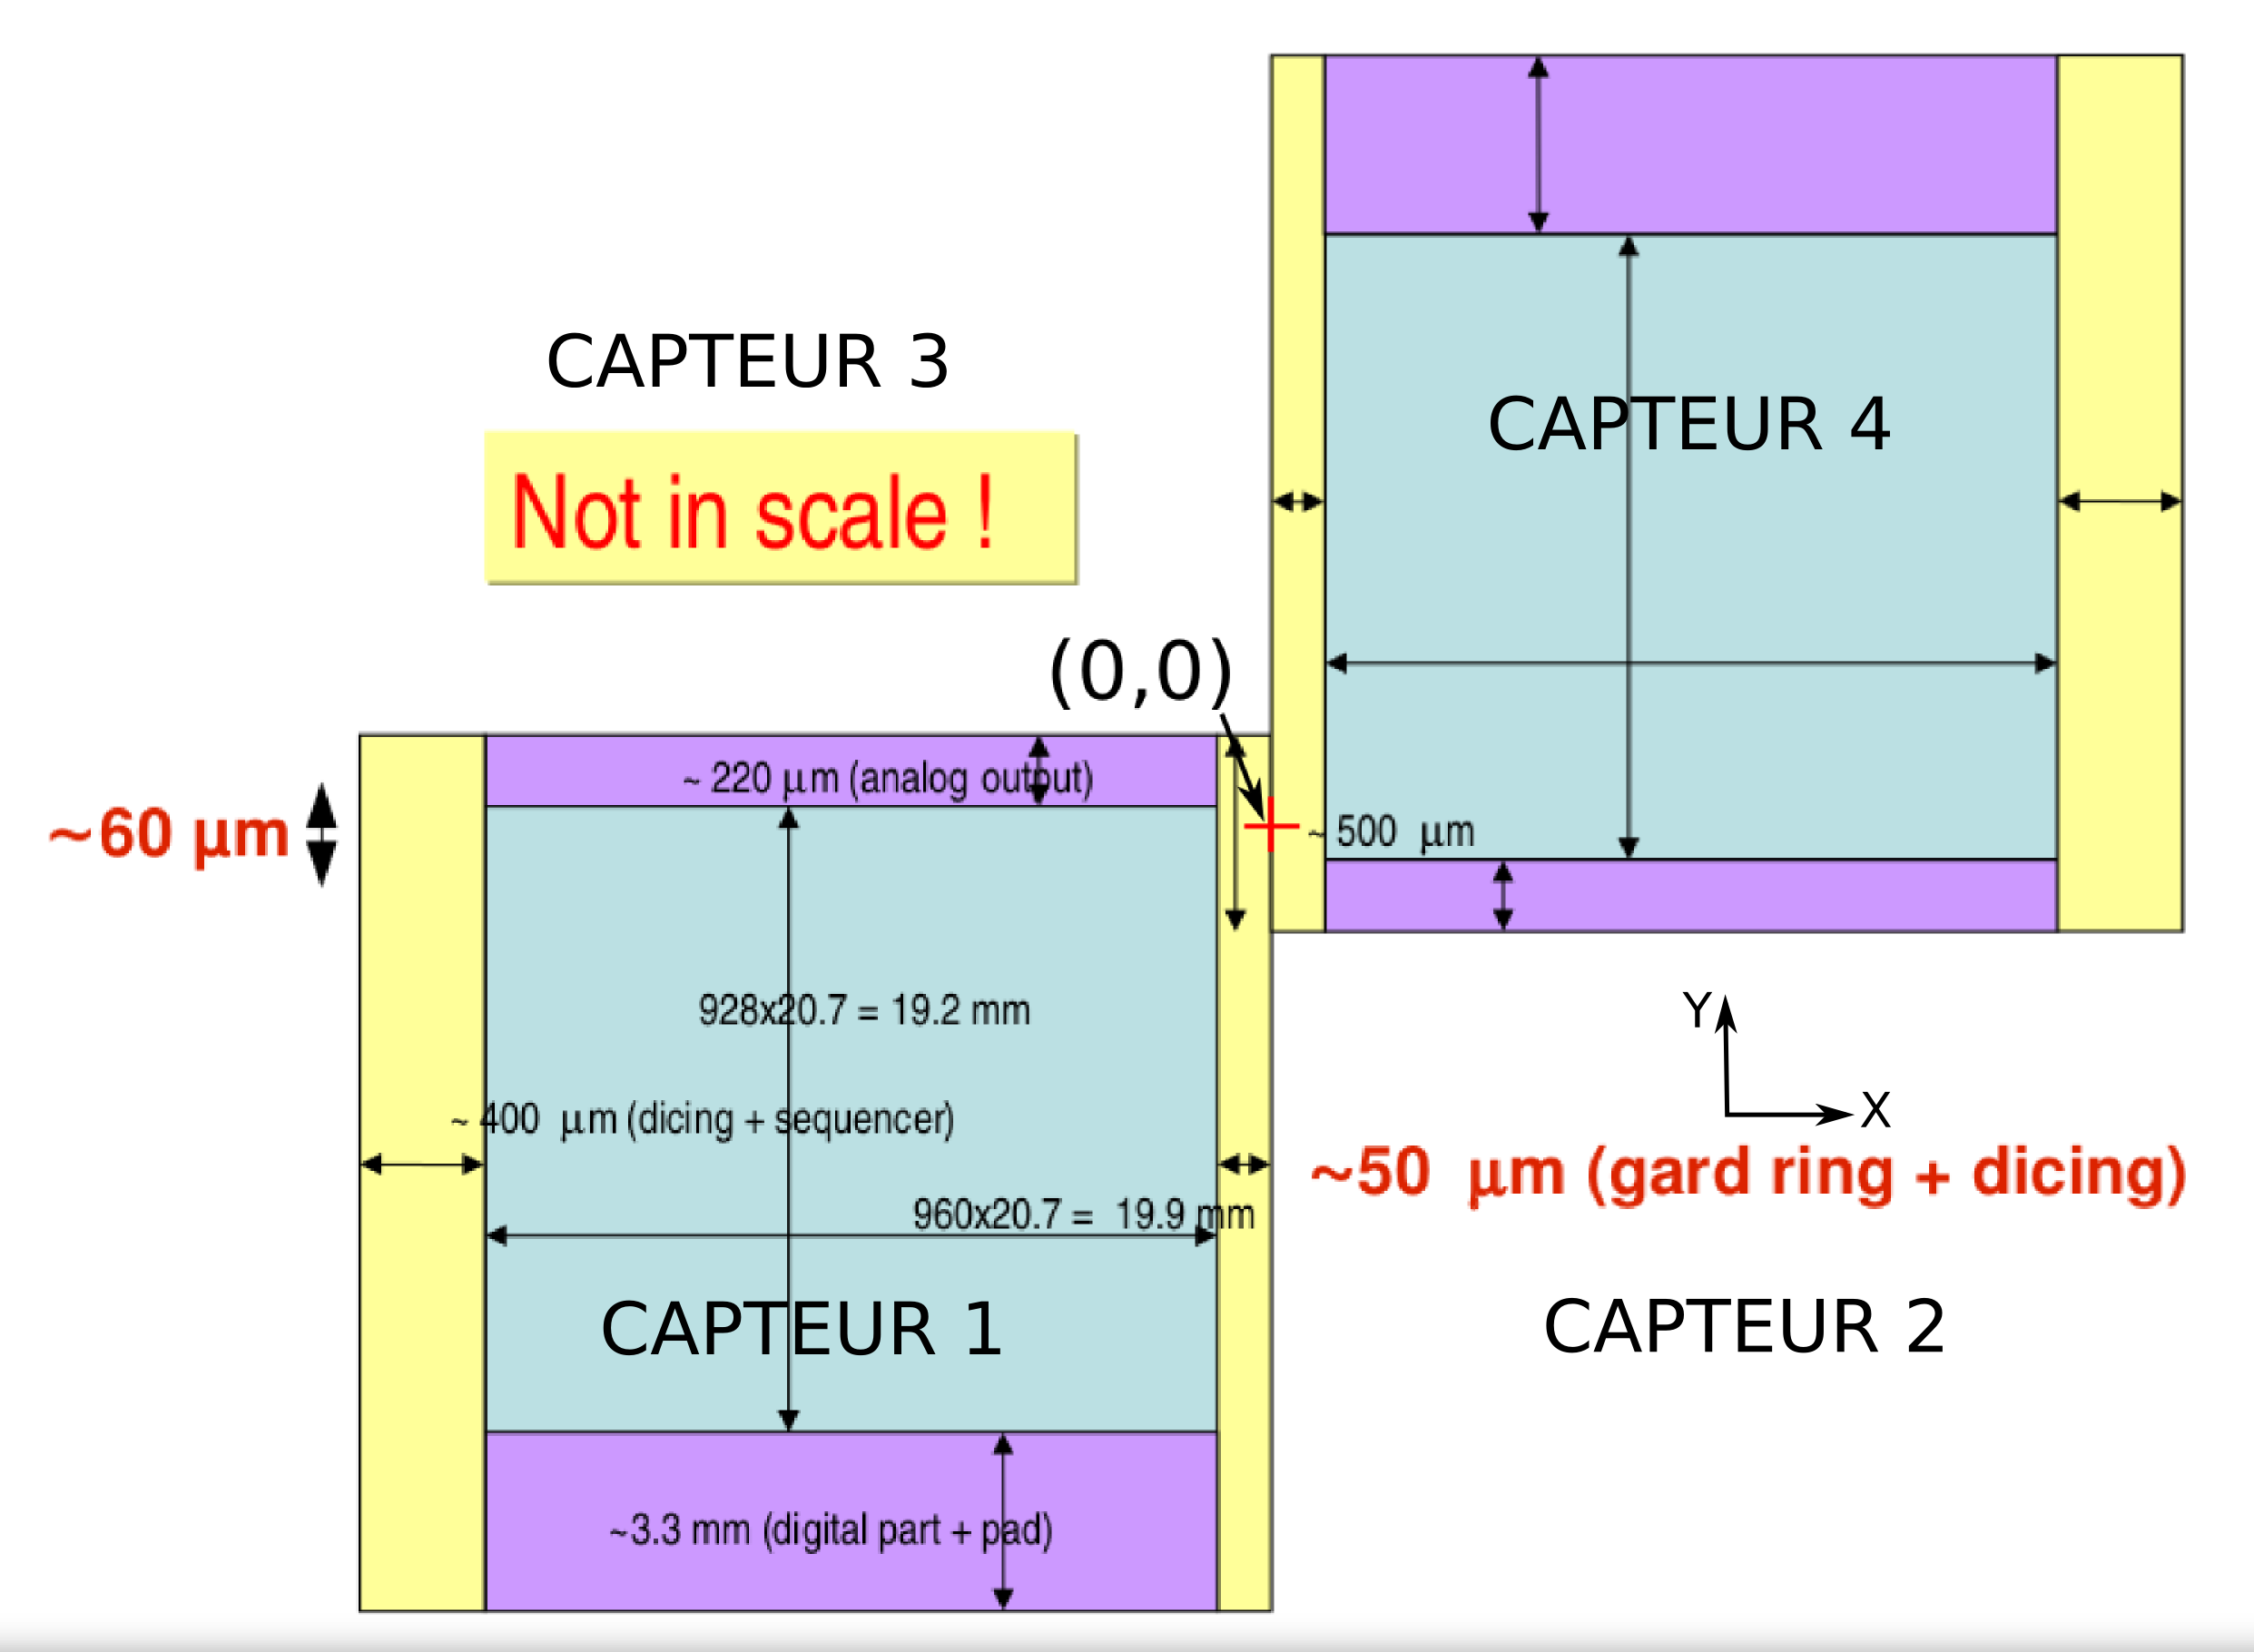
\includegraphics[scale=0.20]{./figures/SALAT_schema.png}
      \caption{Schéma d'un super plan SALAT, vu par la face avant.}
      \label{fig:coordCapteurSALAT00}
   \end{center}
   \end{figure} 
    
  \medskip
    
    La figure \ref{fig:coordCapteurSALAT00} montre la g\'eom\'etrie pour les deux plans de la face avant et montre la position des capteurs 2 et 3 situ\'es sur la face arri\`ere du super-plan. Les axes $X$ et $Y$ et l'origine $O$ sont d\'efinis sur cette figure. Comme indiqu\'e sur cette m\^eme figure les capteurs 1 et 3 et 2 et 4 ont une zone de recouvrement selon l'axe Y de $60 \, \mu m$. Les capteurs 1 et 2 et 3 et 4 sont quant \`a eux distants de l'axe X de $\pm 50 \, \mu m$ par rapport au centre du super plan. On se r\'ef\'erera \`a la figure pour le signe de ce d\'ecalage.
    
  \medskip
   
   Au niveau des inclinaisons, nous allons d\'ecrire les inclinaisons des autres capteurs par rapport au capteur 1 d\'efini sans aucune inclinaison. Le capteur 2 est inclin\'e de 180 degr\'es par rapport \`a son axe vertical $V$. Le capteur 3 est retourn\'e de 180 degr\'es selon son axe horizontal $U$. Enfin, le capteur 4 est inclin\'e de 180 degr\'es suivant son axe horizontal $U$ et de 180 degr\'es suivant son axe vertical $V$. Ainsi, la face pix\'elis\'ee des capteurs 1 et 4 est orient\'ee vers les $z$ n\'egatifs et celle des capteurs 2 et 3 est orient\'ee vers les $z$ positifs.
  
  \subsection{Cible}

  Le t\'elescope en faisceau AIDA sera dot\'e d'une cible afin de g\'en\'erer des vertex. Ceux-ci seront cr\'e\'es \`a la suite des interactions entre les particules du faisceau et la cible. La cible n'a pas \'et\'e \'etudi\'ee lors de cette th\`ese.
  
  \subsection{PLUME}

  Dans ce chapitre, nous avons explicit\'e les avantages des capteurs CMOS. Nous avons soulign\'e leur r\'esolution spatiale avantageuse de l'ordre de quelques microns, coupl\'ee \`a une \'epaisseur tr\`es faible, r\'eduisant ainsi le budget de mati\`ere. Ces caract\'eristiques avantageuses sont combin\'ees \`a une architecture de lecture en volet roulant, permettant un temps de lecture pour un capteur de l'ordre de $200  \, \mu s$ et une dissipation thermique tr\`es inf\'erieure au $W/cm^2$. Pour former un d\'etecteur de vertex \`a base de capteur CMOS, le d\'efi r\'eside dans l'int\'egration de ces capteurs. L'objectif est de construire un d\'etecteur de vertex disposant d'une stabilit\'e m\'ecanique suffisante associ\'ee \`a un budget de mati\`ere r\'eduit. Le projet \textit{PLUME} pour \textit{Pixelated Ladder with Ultra-low Material Embedding} r\'epond \`a cette probl\'ematique en int\'egrant deux couches de capteurs sur un m\^eme support.
  
  \medskip
  
   \begin{figure}[!htb]
    \begin{center} 
     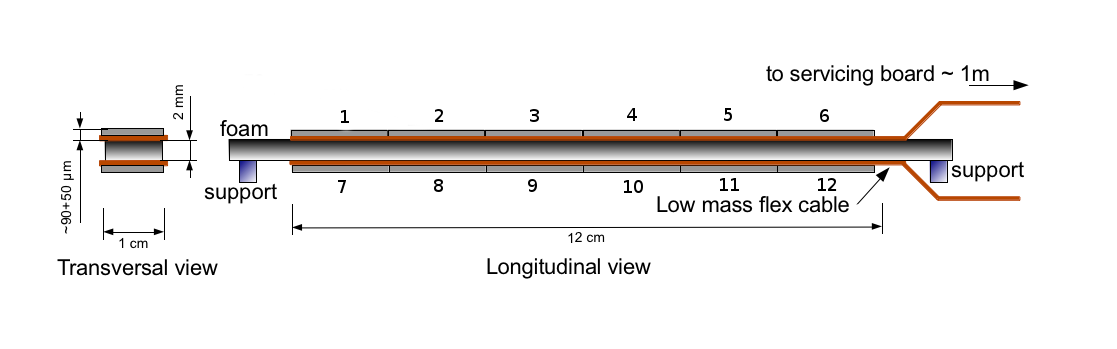
\includegraphics[scale=0.50]{./figures/plume_schema.png}
     \caption{Schéma d'une \'echelle PLUME.}
     \label{fig:PLUME}
    \end{center}
  \end{figure}
  
  La figure \ref{fig:PLUME} illustre les diff\'erents \'el\'ements d'une \'echelle PLUME. Une mousse de carbure de silicium d'une densit\'e de $8 \%$ et \'epaisse de $2 \, mm$ assure la stabilit\'e m\'ecanique de l'\'echelle. Sur chaque face de cette mousse un câble multi-pistes est coll\'e. Il g\`ere les entr\'ees/sorties des capteurs et est constitu\'e de deux couches de pistes en aluminium enrob\'ees d'un polyamide de type Kapton. Les 12 capteurs de l'\'echelle, six par face, sont coll\'es et connect\'es \'electriquement \`a ces câbles. Les câbles des \'echelles \textit{PLUME} pr\'esent\'es ici sont conçus pour pouvoir accueillir des capteurs de type \textit{MIMOSA-26}. Le premier prototype compos\'e de 12 capteurs MIMOSA-26 et pourvu d'un budget de mati\`ere d'environ $0.6\% \, X0$ a vu le jour en 2011 \cite{Baudot:2012mg}. Une photographie de cette \'echelle est visible en figure \ref{fig:PLUME_photo}.
  
  \begin{figure}[!htb]
    \begin{center} 
     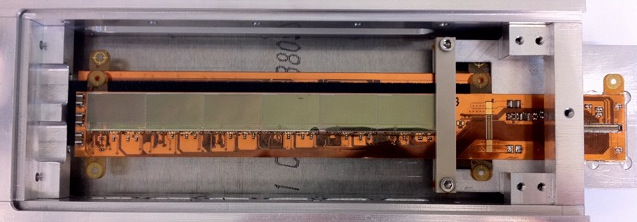
\includegraphics[scale=0.60]{./figures/plume_ladder2010_M26_inBox.jpg}
     \caption{Photographie d'une \'echelle PLUME.}
     \label{fig:PLUME_photo}
    \end{center}
  \end{figure}
  
  \medskip
  
  Le projet \textit{PLUME} permet d'\'etudier la faisabilit\'e technique de ce type d'\'echelles et permet d'explorer la valeur ajout\'ee des \'echelles double faces. Lorsqu'une particule charg\'ee traverse l'\'echelle, un coup par face est cr\'e\'e dans une fenêtre temporelle r\'eduite. L'association de ces deux coups forme un \textit{mini-vecteur}. Ce type d'objet pourrait permettre une meilleure association trace-impact et fournir une nouvelle m\'ethode d'alignement pour des \'echelles double face composant une couche de d\'etecteur de vertex.
  
  \medskip
  
  Un prototype d'\'echelle \textit{PLUME} a ainsi \'et\'e test\'e en Novembre 2011 au SPS. L'objectif de ces tests en faisceaux était la validation et la caract\'erisation de la premi\`ere \'echelle \textit{PLUME} ainsi que le gain apport\'e par les mini-vecteurs sur la r\'esolution spatiale. Nous livrerons les r\'esultats de ces tests en faisceau dans le prochain chapitre.
  
  \subsection{AID Box}
  
  La boite \textit{AID} (\textit{Alignment Investigation Devices}) du t\'elescope \textit{AIDA} accueillera un secteur de d\'etecteur de vertex compos\'e d'un syst\`eme d'\'echelles de capteurs. Ainsi, des \'echelles doubles faces de capteurs pourront \^etre test\'ees en condition r\'eelles. En particulier, des \'echelles \textit{PLUME} pourront \^etre utilis\'ees dans la boîte AID. Ce secteur de d\'etecteur de vertex servira \`a l'\'etude de l'alignement et de la trajectom\'etrie. En particulier, il permettra des \'etudes bas\'ees sur des \'echelles doubles faces \textit{PLUME}. Le passage du faisceau à travers la cible engendre des vertex qui pourront \^etre reconstruits grâce aux traces reconstruites associ\'ees aux vertex dans la boîte \textit{AID}. Des \'etudes d'alignement entre \'echelles doubles faces adjacentes ou entre les diff\'erentes couches d'\'echelles pourront \^etre entreprises. Elles permettront en particulier de valider les techniques d'alignement bas\'ees sur les mini-vecteurs d\'evelopp\'ees dans cette th\`ese. La trajectom\'etrie pourra de plus \^etre \'etudi\'ee, qu'elle soit bas\'ee sur les mini-vecteurs ou sur des techniques plus traditionnelles. Nous \'etudierons dans cette th\`ese des configurations bas\'ees sur des \'echelles doubles faces PLUME.
  
%   Les vertex pourront de plus \^etre reconstruits \`a partir des traces reconstruites dans la boite AID.
% L'objectif étant de simuler les conditions r\'eelles d'un détecteur de vertex en fonctionnement

  \begin{figure}[!htb]
    \begin{center} 
      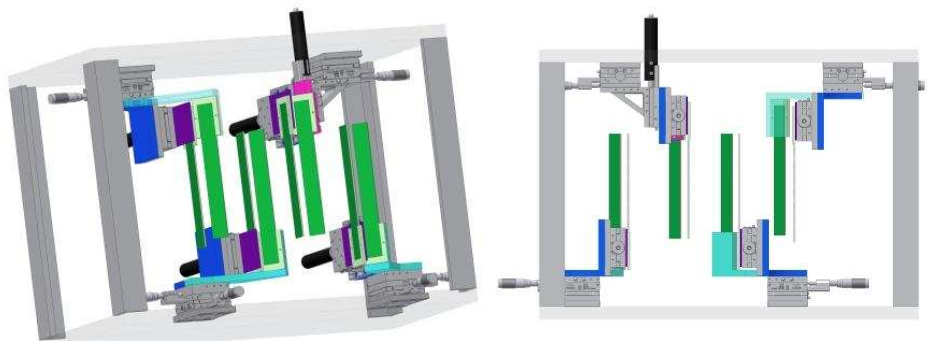
\includegraphics[scale=0.40]{./figures/AID_design.png}
      \caption{Une des repr\'esentations possible pour la boite AID.}
      \label{fig:AID_design}
    \end{center}
  \end{figure}
  
  \section{Conclusion}
  
  Au cours de ce chapitre nous avons relat\'e les caract\'eristiques des capteurs CMOS d\'evelopp\'es par le groupe \textit{PICSEL} pour l'ILD mais aussi pour diff\'erents t\'elescopes en faisceau. Nous avons ensuite d\'ecrit le projet du télescope en faisceau AIDA qui permettra le développement des trajectom\`etres de demain. Nous avons alors mentionn\'e les apports du groupe \textit{PICSEL} \`a la conception de ce t\'elescope. Nous avons notamment d\'ecrit les \'echelles double face \textit{PLUME} et le bras de t\'elescope \textit{SALAT}. L'objectif de cette th\`ese se place dans le d\'eveloppement d'un algorithme d'alignement d\'eveloppé autour du concept de mini-vecteurs. Comme nous l'avons vu la reconstruction de mini-vecteurs est permise par le concept d'\'echelles double face. Dans le prochain chapitre de cette th\`ese nous pr\'esenterons les r\'esultats des tests en faisceau d'une \'echelle PLUME et d'un super-plan SALAT. Puis nous nous focaliserons sur la conception d'une simulation num\'erique d'\'echelles double face de type \textit{PLUME}. Enfin, dans le dernier chapitre, nous utiliserons nos simulations d'\'echelles \textit{PLUME} pour r\'ealiser une m\'ethode d'alignement d'\'echelles double face successives plac\'ees sur une m\^eme couche de d\'etecteur de vertex, gr\^ace aux mini-vecteurs reconstruits \`a l'int\'erieur de leur zone de recouvrement.